% Options for packages loaded elsewhere
\PassOptionsToPackage{unicode}{hyperref}
\PassOptionsToPackage{hyphens}{url}
%
\documentclass[
]{article}
\usepackage{lmodern}
\usepackage{amssymb,amsmath}
\usepackage{ifxetex,ifluatex}
\ifnum 0\ifxetex 1\fi\ifluatex 1\fi=0 % if pdftex
  \usepackage[T1]{fontenc}
  \usepackage[utf8]{inputenc}
  \usepackage{textcomp} % provide euro and other symbols
\else % if luatex or xetex
  \usepackage{unicode-math}
  \defaultfontfeatures{Scale=MatchLowercase}
  \defaultfontfeatures[\rmfamily]{Ligatures=TeX,Scale=1}
\fi
% Use upquote if available, for straight quotes in verbatim environments
\IfFileExists{upquote.sty}{\usepackage{upquote}}{}
\IfFileExists{microtype.sty}{% use microtype if available
  \usepackage[]{microtype}
  \UseMicrotypeSet[protrusion]{basicmath} % disable protrusion for tt fonts
}{}
\makeatletter
\@ifundefined{KOMAClassName}{% if non-KOMA class
  \IfFileExists{parskip.sty}{%
    \usepackage{parskip}
  }{% else
    \setlength{\parindent}{0pt}
    \setlength{\parskip}{6pt plus 2pt minus 1pt}}
}{% if KOMA class
  \KOMAoptions{parskip=half}}
\makeatother
\usepackage{xcolor}
\IfFileExists{xurl.sty}{\usepackage{xurl}}{} % add URL line breaks if available
\IfFileExists{bookmark.sty}{\usepackage{bookmark}}{\usepackage{hyperref}}
\hypersetup{
  pdftitle={Summary of PICRUSt2 analysis of the PET plastisphere},
  hidelinks,
  pdfcreator={LaTeX via pandoc}}
\urlstyle{same} % disable monospaced font for URLs
\usepackage[margin=1in]{geometry}
\usepackage{color}
\usepackage{fancyvrb}
\newcommand{\VerbBar}{|}
\newcommand{\VERB}{\Verb[commandchars=\\\{\}]}
\DefineVerbatimEnvironment{Highlighting}{Verbatim}{commandchars=\\\{\}}
% Add ',fontsize=\small' for more characters per line
\usepackage{framed}
\definecolor{shadecolor}{RGB}{248,248,248}
\newenvironment{Shaded}{\begin{snugshade}}{\end{snugshade}}
\newcommand{\AlertTok}[1]{\textcolor[rgb]{0.94,0.16,0.16}{#1}}
\newcommand{\AnnotationTok}[1]{\textcolor[rgb]{0.56,0.35,0.01}{\textbf{\textit{#1}}}}
\newcommand{\AttributeTok}[1]{\textcolor[rgb]{0.77,0.63,0.00}{#1}}
\newcommand{\BaseNTok}[1]{\textcolor[rgb]{0.00,0.00,0.81}{#1}}
\newcommand{\BuiltInTok}[1]{#1}
\newcommand{\CharTok}[1]{\textcolor[rgb]{0.31,0.60,0.02}{#1}}
\newcommand{\CommentTok}[1]{\textcolor[rgb]{0.56,0.35,0.01}{\textit{#1}}}
\newcommand{\CommentVarTok}[1]{\textcolor[rgb]{0.56,0.35,0.01}{\textbf{\textit{#1}}}}
\newcommand{\ConstantTok}[1]{\textcolor[rgb]{0.00,0.00,0.00}{#1}}
\newcommand{\ControlFlowTok}[1]{\textcolor[rgb]{0.13,0.29,0.53}{\textbf{#1}}}
\newcommand{\DataTypeTok}[1]{\textcolor[rgb]{0.13,0.29,0.53}{#1}}
\newcommand{\DecValTok}[1]{\textcolor[rgb]{0.00,0.00,0.81}{#1}}
\newcommand{\DocumentationTok}[1]{\textcolor[rgb]{0.56,0.35,0.01}{\textbf{\textit{#1}}}}
\newcommand{\ErrorTok}[1]{\textcolor[rgb]{0.64,0.00,0.00}{\textbf{#1}}}
\newcommand{\ExtensionTok}[1]{#1}
\newcommand{\FloatTok}[1]{\textcolor[rgb]{0.00,0.00,0.81}{#1}}
\newcommand{\FunctionTok}[1]{\textcolor[rgb]{0.00,0.00,0.00}{#1}}
\newcommand{\ImportTok}[1]{#1}
\newcommand{\InformationTok}[1]{\textcolor[rgb]{0.56,0.35,0.01}{\textbf{\textit{#1}}}}
\newcommand{\KeywordTok}[1]{\textcolor[rgb]{0.13,0.29,0.53}{\textbf{#1}}}
\newcommand{\NormalTok}[1]{#1}
\newcommand{\OperatorTok}[1]{\textcolor[rgb]{0.81,0.36,0.00}{\textbf{#1}}}
\newcommand{\OtherTok}[1]{\textcolor[rgb]{0.56,0.35,0.01}{#1}}
\newcommand{\PreprocessorTok}[1]{\textcolor[rgb]{0.56,0.35,0.01}{\textit{#1}}}
\newcommand{\RegionMarkerTok}[1]{#1}
\newcommand{\SpecialCharTok}[1]{\textcolor[rgb]{0.00,0.00,0.00}{#1}}
\newcommand{\SpecialStringTok}[1]{\textcolor[rgb]{0.31,0.60,0.02}{#1}}
\newcommand{\StringTok}[1]{\textcolor[rgb]{0.31,0.60,0.02}{#1}}
\newcommand{\VariableTok}[1]{\textcolor[rgb]{0.00,0.00,0.00}{#1}}
\newcommand{\VerbatimStringTok}[1]{\textcolor[rgb]{0.31,0.60,0.02}{#1}}
\newcommand{\WarningTok}[1]{\textcolor[rgb]{0.56,0.35,0.01}{\textbf{\textit{#1}}}}
\usepackage{graphicx,grffile}
\makeatletter
\def\maxwidth{\ifdim\Gin@nat@width>\linewidth\linewidth\else\Gin@nat@width\fi}
\def\maxheight{\ifdim\Gin@nat@height>\textheight\textheight\else\Gin@nat@height\fi}
\makeatother
% Scale images if necessary, so that they will not overflow the page
% margins by default, and it is still possible to overwrite the defaults
% using explicit options in \includegraphics[width, height, ...]{}
\setkeys{Gin}{width=\maxwidth,height=\maxheight,keepaspectratio}
% Set default figure placement to htbp
\makeatletter
\def\fps@figure{htbp}
\makeatother
\setlength{\emergencystretch}{3em} % prevent overfull lines
\providecommand{\tightlist}{%
  \setlength{\itemsep}{0pt}\setlength{\parskip}{0pt}}
\setcounter{secnumdepth}{-\maxdimen} % remove section numbering
\usepackage{booktabs}
\usepackage{longtable}
\usepackage{array}
\usepackage{multirow}
\usepackage{wrapfig}
\usepackage{float}
\usepackage{colortbl}
\usepackage{pdflscape}
\usepackage{tabu}
\usepackage{threeparttable}
\usepackage{threeparttablex}
\usepackage[normalem]{ulem}
\usepackage{makecell}
\usepackage{xcolor}

\title{Summary of PICRUSt2 analysis of the PET plastisphere}
\author{}
\date{\vspace{-2.5em}}

\begin{document}
\maketitle

{
\setcounter{tocdepth}{2}
\tableofcontents
}
\begin{Shaded}
\begin{Highlighting}[]
\ImportTok{import}\NormalTok{ os}
\ImportTok{import}\NormalTok{ pandas }\ImportTok{as}\NormalTok{ pd}
\ImportTok{import}\NormalTok{ csv}
\ImportTok{import}\NormalTok{ numpy }\ImportTok{as}\NormalTok{ np}
\ImportTok{import}\NormalTok{ math}
\ImportTok{from}\NormalTok{ matplotlib.lines }\ImportTok{import}\NormalTok{ Line2D}
\ImportTok{import}\NormalTok{ matplotlib }\ImportTok{as}\NormalTok{ mpl}
\ImportTok{from}\NormalTok{ matplotlib.patches }\ImportTok{import}\NormalTok{ Patch}
\ImportTok{import}\NormalTok{ matplotlib.pyplot }\ImportTok{as}\NormalTok{ plt}
\ImportTok{import}\NormalTok{ random}
\ImportTok{from}\NormalTok{ scipy.spatial }\ImportTok{import}\NormalTok{ distance}
\ImportTok{from}\NormalTok{ scipy }\ImportTok{import}\NormalTok{ stats}
\ImportTok{from}\NormalTok{ sklearn }\ImportTok{import}\NormalTok{ manifold}
\ImportTok{from}\NormalTok{ sklearn.decomposition }\ImportTok{import}\NormalTok{ PCA}
\ImportTok{import}\NormalTok{ statsmodels.stats.multitest }\ImportTok{as}\NormalTok{ sm}
\ImportTok{from}\NormalTok{ mpl_toolkits.axes_grid1 }\ImportTok{import}\NormalTok{ make_axes_locatable}
\end{Highlighting}
\end{Shaded}

\hypertarget{summary}{%
\section{Summary}\label{summary}}

Here I have several sections showing an exploration of genes for PET
degradation present in the PICRUSt2 predicted metagenomes.

\hypertarget{genes-included}{%
\subsection{Genes included}\label{genes-included}}

Summary of the genes that we are looking for in the predicted
metagenomes.

\begin{Shaded}
\begin{Highlighting}[]
\NormalTok{cols }\OperatorTok{=}\NormalTok{ [}\StringTok{'KEGG ortholog'}\NormalTok{, }\StringTok{'Product'}\NormalTok{, }\StringTok{'Added to PICRUSt2'}\NormalTok{]}
\NormalTok{genes }\OperatorTok{=}\NormalTok{ [[}\StringTok{'K21104'}\NormalTok{, }\StringTok{'Poly(ethylene terephthalate) hydrolase (PETase)'}\NormalTok{, }\StringTok{'HMM'}\NormalTok{], [}\StringTok{'K18074'}\NormalTok{, }\StringTok{'Terephthalate 1,2-dioxygenase oxygenase component (alpha subunit; tphA2)'}\NormalTok{, }\StringTok{'HMM'}\NormalTok{], [}\StringTok{'K18074'}\NormalTok{, }\StringTok{'Terephthalate 1,2-dioxygenase oxygenase component (alpha subunit; tphA3)'}\NormalTok{, }\StringTok{'HMM'}\NormalTok{], [}\StringTok{'K18076'}\NormalTok{, }\StringTok{'1,2-dihydroxy-3,5-cyclohexadiene-1,4-dicarboxylate dehydrogenase (tphB)'}\NormalTok{, }\StringTok{'HMM'}\NormalTok{], [}\StringTok{'K00448'}\NormalTok{, }\StringTok{'Protocatechuate 3,4-dioxygenase (alpha subunit; pcaG)'}\NormalTok{, }\StringTok{'Default'}\NormalTok{], [}\StringTok{'K00449'}\NormalTok{, }\StringTok{'Protocatechuate 3,4- dioxygenase (beta subunit; pcaH)'}\NormalTok{, }\StringTok{'Default'}\NormalTok{], [}\StringTok{'K01857'}\NormalTok{, }\StringTok{'3-carboxy-cis,cis-muconate cycloisomerase (pcaB)'}\NormalTok{, }\StringTok{'Default'}\NormalTok{], [}\StringTok{'K01607'}\NormalTok{, }\StringTok{'4-carboxymuconolactone decarboxylase (pcaC)'}\NormalTok{, }\StringTok{'Default'}\NormalTok{], [}\StringTok{'K14727'}\NormalTok{, }\StringTok{'3-oxoadipate enol-lactonase / 4-carboxymuconolactone decarboxylase (pcaL)'}\NormalTok{, }\StringTok{'Default'}\NormalTok{], [}\StringTok{'K01055'}\NormalTok{, }\StringTok{'3-oxoadipate enol-lactonase (pcaD)'}\NormalTok{, }\StringTok{'Default'}\NormalTok{], [}\StringTok{'K01031'}\NormalTok{, }\StringTok{'3-oxoadipate CoA-transferase (alpha subunit; pcaI)'}\NormalTok{, }\StringTok{'Default'}\NormalTok{], [}\StringTok{'K01032'}\NormalTok{, }\StringTok{'3-oxoadipate CoA-transferase (beta subunit; pcaJ)'}\NormalTok{, }\StringTok{'Default'}\NormalTok{]]}
\NormalTok{genes_df }\OperatorTok{=}\NormalTok{ pd.DataFrame(genes, columns}\OperatorTok{=}\NormalTok{cols)}
\NormalTok{genes_df }\OperatorTok{=}\NormalTok{ genes_df.set_index(}\StringTok{'KEGG ortholog'}\NormalTok{)}
\end{Highlighting}
\end{Shaded}

\begin{Shaded}
\begin{Highlighting}[]
\NormalTok{py}\OperatorTok{$}\NormalTok{genes_df }\OperatorTok
\StringTok{  }\KeywordTok{kable}\NormalTok{() }\OperatorTok
\StringTok{  }\KeywordTok{kable_styling}\NormalTok{()}
\end{Highlighting}
\end{Shaded}

\begin{verbatim}
## Warning in py_to_r.pandas.core.frame.DataFrame(x): index contains duplicated
## values: row names not set
\end{verbatim}

\begin{table}[H]
\centering
\begin{tabular}{l|l}
\hline
Product & Added to PICRUSt2\\
\hline
Poly(ethylene terephthalate) hydrolase (PETase) & HMM\\
\hline
Terephthalate 1,2-dioxygenase oxygenase component (alpha subunit; tphA2) & HMM\\
\hline
Terephthalate 1,2-dioxygenase oxygenase component (alpha subunit; tphA3) & HMM\\
\hline
1,2-dihydroxy-3,5-cyclohexadiene-1,4-dicarboxylate dehydrogenase (tphB) & HMM\\
\hline
Protocatechuate 3,4-dioxygenase (alpha subunit; pcaG) & Default\\
\hline
Protocatechuate 3,4- dioxygenase (beta subunit; pcaH) & Default\\
\hline
3-carboxy-cis,cis-muconate cycloisomerase (pcaB) & Default\\
\hline
4-carboxymuconolactone decarboxylase (pcaC) & Default\\
\hline
3-oxoadipate enol-lactonase / 4-carboxymuconolactone decarboxylase (pcaL) & Default\\
\hline
3-oxoadipate enol-lactonase (pcaD) & Default\\
\hline
3-oxoadipate CoA-transferase (alpha subunit; pcaI) & Default\\
\hline
3-oxoadipate CoA-transferase (beta subunit; pcaJ) & Default\\
\hline
\end{tabular}
\end{table}

\hypertarget{petases-predicted}{%
\subsection{PETases predicted}\label{petases-predicted}}

Look at the ASVs predicted to contain PETases and their taxonomic
classifications. Note that many of these ASVs are currently unclassified
at even the phylum level.

\begin{Shaded}
\begin{Highlighting}[]
\NormalTok{petases }\OperatorTok{=}\NormalTok{ pd.read_csv(}\StringTok{'/Users/robynwright/Documents/OneDrive/Github/PET-plastisphere-community/PICRUSt2/results/picrust_not_reduced/ko_PETases.csv'}\NormalTok{, header}\OperatorTok{=}\VariableTok{None}\NormalTok{, index_col}\OperatorTok{=}\DecValTok{0}\NormalTok{)}
\CommentTok{#print(petases.loc['ASV000020', :].values[0])}
\NormalTok{asvs }\OperatorTok{=} \BuiltInTok{list}\NormalTok{(petases.index.values)}
\NormalTok{copies }\OperatorTok{=} \BuiltInTok{list}\NormalTok{(petases.loc[:, }\DecValTok{1}\NormalTok{])}

\NormalTok{abun }\OperatorTok{=}\NormalTok{ pd.read_csv(}\StringTok{'/Users/robynwright/Documents/OneDrive/PhD_Plastic_Oceans/Experiments/PET_MiSeq2/basic/Treatment1_All_percent.csv'}\NormalTok{, index_col}\OperatorTok{=}\DecValTok{0}\NormalTok{, header}\OperatorTok{=}\DecValTok{0}\NormalTok{)}

\NormalTok{taxonomy }\OperatorTok{=}\NormalTok{ pd.read_csv(}\StringTok{'/Users/robynwright/Documents/OneDrive/PhD_Plastic_Oceans/Experiments/PET_MiSeq2/basic/Taxonomy.csv'}\NormalTok{, header}\OperatorTok{=}\DecValTok{0}\NormalTok{, index_col}\OperatorTok{=}\DecValTok{0}\NormalTok{)}
\NormalTok{taxonomy }\OperatorTok{=}\NormalTok{ taxonomy.loc[asvs, :]}
\NormalTok{labels }\OperatorTok{=}\NormalTok{ [}\StringTok{'Kingdom'}\NormalTok{, }\StringTok{'Phylum'}\NormalTok{, }\StringTok{'Class'}\NormalTok{, }\StringTok{'Order'}\NormalTok{, }\StringTok{'Family'}\NormalTok{, }\StringTok{'Genus'}\NormalTok{, }\StringTok{'Species'}\NormalTok{]}
\NormalTok{maxs, maxs_trt }\OperatorTok{=}\NormalTok{ [], []}
\ControlFlowTok{for}\NormalTok{ asv }\KeywordTok{in}\NormalTok{ asvs:}
\NormalTok{  this_asv }\OperatorTok{=}\NormalTok{ taxonomy.loc[asv, :].values}
  \ControlFlowTok{for}\NormalTok{ b }\KeywordTok{in} \BuiltInTok{range}\NormalTok{(}\BuiltInTok{len}\NormalTok{(this_asv)):}
    \ControlFlowTok{if} \KeywordTok{not} \BuiltInTok{isinstance}\NormalTok{(this_asv[b], }\BuiltInTok{str}\NormalTok{):}
      \ControlFlowTok{if}\NormalTok{ b }\OperatorTok{==} \DecValTok{6} \KeywordTok{and} \StringTok{'Unclassified'} \KeywordTok{not} \KeywordTok{in}\NormalTok{ this_asv[b}\DecValTok{-1}\NormalTok{]:}
\NormalTok{        new }\OperatorTok{=}\NormalTok{ this_asv[b}\DecValTok{-1}\NormalTok{]}\OperatorTok{+}\StringTok{' sp.'}
      \ControlFlowTok{elif} \StringTok{'Unclassified'} \KeywordTok{not} \KeywordTok{in}\NormalTok{ this_asv[b}\DecValTok{-1}\NormalTok{]:}
\NormalTok{        new }\OperatorTok{=} \StringTok{'Unclassified '}\OperatorTok{+}\NormalTok{this_asv[b}\DecValTok{-1}\NormalTok{]}
      \ControlFlowTok{else}\NormalTok{:}
\NormalTok{        new }\OperatorTok{=}\NormalTok{ this_asv[b}\DecValTok{-1}\NormalTok{]}
\NormalTok{      taxonomy.loc[asv, labels[b]] }\OperatorTok{=}\NormalTok{ new}
    \ControlFlowTok{elif}\NormalTok{ b }\OperatorTok{==} \DecValTok{6} \KeywordTok{and} \BuiltInTok{isinstance}\NormalTok{(this_asv[b], }\BuiltInTok{str}\NormalTok{):}
\NormalTok{      taxonomy.loc[asv, labels[b]] }\OperatorTok{=}\NormalTok{ this_asb[b}\DecValTok{-1}\NormalTok{]}\OperatorTok{+}\StringTok{' '}\OperatorTok{+}\NormalTok{this_asv[b]}
\NormalTok{  maximum }\OperatorTok{=}\NormalTok{ abun.loc[asv, :].}\BuiltInTok{max}\NormalTok{(axis}\OperatorTok{=}\DecValTok{0}\NormalTok{)}
\NormalTok{  maximum_id }\OperatorTok{=}\NormalTok{ abun.loc[asv, :].idxmax(axis}\OperatorTok{=}\DecValTok{1}\NormalTok{)}
\NormalTok{  maxs.append(maximum), maxs_trt.append(maximum_id)}
\end{Highlighting}
\end{Shaded}

\begin{Shaded}
\begin{Highlighting}[]
\NormalTok{taxonomy.drop([}\StringTok{'Kingdom'}\NormalTok{, }\StringTok{'Phylum'}\NormalTok{, }\StringTok{'Class'}\NormalTok{, }\StringTok{'Order'}\NormalTok{, }\StringTok{'Family'}\NormalTok{, }\StringTok{'Genus'}\NormalTok{], axis}\OperatorTok{=}\DecValTok{1}\NormalTok{, inplace}\OperatorTok{=}\VariableTok{True}\NormalTok{)}
\NormalTok{taxonomy[}\StringTok{'PETase copies'}\NormalTok{] }\OperatorTok{=}\NormalTok{ copies}
\NormalTok{taxonomy[}\StringTok{'Maximum relative abundance (%)'}\NormalTok{] }\OperatorTok{=}\NormalTok{ maxs}
\NormalTok{taxonomy[}\StringTok{'Treatment'}\NormalTok{] }\OperatorTok{=}\NormalTok{ maxs_trt}
\CommentTok{#taxonomy = taxonomy.sort_values(['Class', 'Order', 'Family', 'Genus', 'Species'])}
\NormalTok{taxonomy }\OperatorTok{=}\NormalTok{ taxonomy.sort_values([}\StringTok{'Maximum relative abundance (%)'}\NormalTok{], ascending}\OperatorTok{=}\VariableTok{False}\NormalTok{)}
\end{Highlighting}
\end{Shaded}

\begin{Shaded}
\begin{Highlighting}[]
\NormalTok{py}\OperatorTok{$}\NormalTok{taxonomy }\OperatorTok
\StringTok{  }\KeywordTok{kable}\NormalTok{() }\OperatorTok
\StringTok{  }\KeywordTok{kable_styling}\NormalTok{()}
\end{Highlighting}
\end{Shaded}

\begin{table}[H]
\centering
\begin{tabular}{l|l|r|r|l}
\hline
  & Species & PETase copies & Maximum relative abundance (\%) & Treatment\\
\hline
ASV000020 & Pseudomonas sp. & 2 & 12.4684821 & Day42PET2\\
\hline
ASV000043 & Azomonas sp. & 2 & 4.3419379 & Day14WeatherPET1\\
\hline
ASV000098 & Unclassified Gammaproteobacteria & 2 & 1.1860303 & Day14WeatherPET1\\
\hline
ASV000272 & Pseudomonas sp. & 2 & 0.8623088 & Day42WeatherPET2\\
\hline
ASV000126 & Azomonas sp. & 2 & 0.5006771 & Day14WeatherPET1\\
\hline
ASV000610 & Unclassified Rhodobacteraceae & 1 & 0.0762311 & Inoc4\\
\hline
ASV000486 & Unclassified Pseudonocardiaceae & 2 & 0.0731886 & Day21WeatherPET3\\
\hline
ASV000859 & Azomonas sp. & 2 & 0.0575374 & Day30WeatherPET1\\
\hline
ASV000621 & Unclassified Pseudomonadaceae & 2 & 0.0533508 & Day14WeatherPET1\\
\hline
ASV002089 & Marinobacter sp. & 2 & 0.0508259 & Day07PET1\\
\hline
ASV001854 & Azomonas sp. & 2 & 0.0504286 & Day42PET2\\
\hline
ASV002886 & Azomonas sp. & 2 & 0.0460299 & Day30WeatherPET1\\
\hline
ASV002319 & Azomonas sp. & 2 & 0.0386274 & Day21WeatherPET1\\
\hline
ASV002444 & Unclassified Rhodobacteraceae & 1 & 0.0376967 & Inoc3\\
\hline
ASV008863 & Unclassified Gammaproteobacteria & 2 & 0.0365943 & Day21WeatherPET3\\
\hline
ASV008860 & Unclassified Pseudomonadaceae & 2 & 0.0365943 & Day21WeatherPET3\\
\hline
ASV009408 & Unclassified Gammaproteobacteria & 2 & 0.0363901 & Day30PET3\\
\hline
ASV001422 & Azomonas sp. & 2 & 0.0359567 & Day30WeatherPET3\\
\hline
ASV005194 & Azomonas sp. & 2 & 0.0345224 & Day30WeatherPET1\\
\hline
ASV006460 & Spongiispira sp. & 1 & 0.0333556 & Inoc1\\
\hline
ASV001694 & Unclassified Rhodobacteraceae & 1 & 0.0333556 & Inoc1\\
\hline
ASV001672 & Unclassified Pseudomonadaceae & 2 & 0.0291015 & Day07WeatherPET3\\
\hline
ASV005178 & Unclassified Gammaproteobacteria & 2 & 0.0288226 & Day30PET1\\
\hline
ASV001181 & Unclassified Pseudonocardiaceae & 2 & 0.0288226 & Day30PET1\\
\hline
ASV006452 & Parvibaculum sp. & 2 & 0.0285103 & Day21PET2\\
\hline
ASV002594 & Azomonas sp. & 2 & 0.0278164 & Day42WeatherPET2\\
\hline
ASV003071 & Azomonas sp. & 2 & 0.0257715 & Day42WeatherPET3\\
\hline
ASV005905 & Unclassified Gammaproteobacteria & 2 & 0.0257715 & Day42WeatherPET3\\
\hline
ASV005761 & Unclassified Pseudomonadaceae & 2 & 0.0252143 & Day42PET2\\
\hline
ASV005789 & Unclassified Pseudomonadaceae & 2 & 0.0252143 & Day42PET2\\
\hline
ASV009940 & Azomonas sp. & 2 & 0.0252143 & Day42PET2\\
\hline
ASV009965 & Azomonas sp. & 2 & 0.0252143 & Day42PET2\\
\hline
ASV009960 & Azomonas sp. & 2 & 0.0252143 & Day42PET2\\
\hline
ASV009947 & Unclassified Alphaproteobacteria & 2 & 0.0252143 & Day42PET2\\
\hline
ASV003868 & Unclassified Micromonosporaceae & 1 & 0.0248433 & Day01ExtractionControl\\
\hline
ASV003774 & Azomonas sp. & 2 & 0.0243962 & Day21WeatherPET3\\
\hline
ASV005219 & Unclassified Cellvibrionales & 2 & 0.0243962 & Day21WeatherPET3\\
\hline
ASV004312 & Oleibacter sp. & 2 & 0.0243843 & Day01LowCrys1\\
\hline
ASV002442 & Azomonas sp. & 2 & 0.0242028 & Day30WeatherPET2\\
\hline
ASV005769 & Azomonas sp. & 2 & 0.0242028 & Day30WeatherPET2\\
\hline
ASV008825 & Unclassified Pseudonocardiaceae & 2 & 0.0236202 & Day21PET3\\
\hline
ASV009426 & Azomonas sp. & 2 & 0.0230150 & Day30WeatherPET1\\
\hline
ASV009448 & Unclassified Rhodobacteraceae & 2 & 0.0230150 & Day30WeatherPET1\\
\hline
ASV002887 & Azomonas sp. & 2 & 0.0222255 & Day14PET2\\
\hline
ASV003511 & Unclassified Proteobacteria & 2 & 0.0218261 & Day07WeatherPET3\\
\hline
ASV008802 & Unclassified Gammaproteobacteria & 2 & 0.0213828 & Day21PET2\\
\hline
ASV008806 & Unclassified Stappiaceae & 2 & 0.0213828 & Day21PET2\\
\hline
ASV001853 & Azomonas sp. & 2 & 0.0205196 & Day14WeatherPET1\\
\hline
ASV007101 & Azomonas sp. & 2 & 0.0193287 & Day42WeatherPET3\\
\hline
ASV002893 & Azomonas sp. & 2 & 0.0193137 & Day21WeatherPET1\\
\hline
ASV003151 & Aliisedimentitalea sp. & 1 & 0.0188484 & Inoc3\\
\hline
ASV014304 & Unclassified Gammaproteobacteria & 2 & 0.0181951 & Day30PET3\\
\hline
ASV014303 & Azomonas sp. & 2 & 0.0181951 & Day30PET3\\
\hline
ASV014290 & Azomonas sp. & 2 & 0.0181951 & Day30PET3\\
\hline
ASV014297 & Azomonas sp. & 2 & 0.0181951 & Day30PET3\\
\hline
ASV006801 & Unclassified Gammaproteobacteria & 2 & 0.0181521 & Day30WeatherPET2\\
\hline
ASV008182 & Azomonas sp. & 2 & 0.0181324 & Day07WeatherPET2\\
\hline
ASV006758 & Unclassified Gammaproteobacteria & 2 & 0.0178010 & Day30PET2\\
\hline
ASV004559 & Aliisedimentitalea sp. & 1 & 0.0170692 & Day01NoC3\\
\hline
ASV003951 & Unclassified Rhodobacteraceae & 1 & 0.0168095 & Day30LowCrysWater3\\
\hline
ASV009972 & Unclassified Gammaproteobacteria & 2 & 0.0163159 & Day42PET3\\
\hline
ASV013647 & Unclassified Gammaproteobacteria & 2 & 0.0157468 & Day21PET3\\
\hline
ASV013603 & Azomonas sp. & 2 & 0.0157468 & Day21PET3\\
\hline
ASV008855 & Unclassified Gammaproteobacteria & 2 & 0.0154544 & Day21WeatherPET2\\
\hline
ASV008847 & Azomonas sp. & 2 & 0.0154544 & Day21WeatherPET2\\
\hline
ASV004316 & Unclassified Frankiales & 1 & 0.0153633 & Day14ExtractionControl\\
\hline
ASV004030 & Unclassified Rhodobacteraceae & 1 & 0.0152462 & Inoc4\\
\hline
ASV002737 & Unclassified Pseudonocardiaceae & 2 & 0.0148170 & Day14PET2\\
\hline
ASV012702 & Unclassified Gammaproteobacteria & 2 & 0.0148170 & Day14PET2\\
\hline
ASV012666 & Unclassified Rhodobacteraceae & 2 & 0.0148170 & Day14PET2\\
\hline
ASV012665 & Unclassified Gammaproteobacteria & 2 & 0.0148170 & Day14PET2\\
\hline
ASV012068 & Unclassified Cellvibrionales & 2 & 0.0145507 & Day07WeatherPET3\\
\hline
ASV012061 & Azomonas sp. & 2 & 0.0145507 & Day07WeatherPET3\\
\hline
ASV012082 & Azomonas sp. & 2 & 0.0145507 & Day07WeatherPET3\\
\hline
ASV005294 & Azomonas sp. & 2 & 0.0145507 & Day07WeatherPET3\\
\hline
ASV012056 & Unclassified Gammaproteobacteria & 2 & 0.0145507 & Day07WeatherPET3\\
\hline
ASV004738 & Unclassified Gammaproteobacteria & 2 & 0.0145507 & Day07WeatherPET3\\
\hline
ASV009119 & Unclassified Pseudonocardiaceae & 2 & 0.0144760 & Day30NoC2\\
\hline
ASV013553 & Azomonas sp. & 2 & 0.0142552 & Day21PET2\\
\hline
ASV013564 & Unclassified Gammaproteobacteria & 2 & 0.0142552 & Day21PET2\\
\hline
ASV013593 & Unclassified Gammaproteobacteria & 2 & 0.0142552 & Day21PET2\\
\hline
ASV009988 & Azomonas sp. & 2 & 0.0139198 & Day42WeatherPET1\\
\hline
ASV009994 & Unclassified Gammaproteobacteria & 2 & 0.0139198 & Day42WeatherPET1\\
\hline
ASV004344 & Azomonas sp. & 2 & 0.0139198 & Day42WeatherPET1\\
\hline
ASV010004 & Azomonas sp. & 2 & 0.0139198 & Day42WeatherPET1\\
\hline
ASV005304 & Unclassified Gammaproteobacteria & 2 & 0.0139082 & Day42WeatherPET2\\
\hline
ASV006826 & Azomonas sp. & 2 & 0.0134838 & Day30WeatherPET3\\
\hline
ASV012910 & Azomonas sp. & 2 & 0.0131087 & Day14WeatherPET3\\
\hline
ASV012904 & Unclassified Gammaproteobacteria & 2 & 0.0131087 & Day14WeatherPET3\\
\hline
ASV012585 & Azomonas sp. & 2 & 0.0128916 & Day14PET1\\
\hline
ASV012633 & Azomonas sp. & 2 & 0.0128916 & Day14PET1\\
\hline
ASV010052 & Unclassified Proteobacteria & 2 & 0.0128858 & Day42WeatherPET3\\
\hline
ASV010061 & Unclassified Gammaproteobacteria & 2 & 0.0128858 & Day42WeatherPET3\\
\hline
ASV013707 & Unclassified Proteobacteria & 2 & 0.0128758 & Day21WeatherPET1\\
\hline
ASV013670 & Unclassified Gammaproteobacteria & 2 & 0.0128758 & Day21WeatherPET1\\
\hline
ASV013658 & Unclassified Alphaproteobacteria & 2 & 0.0128758 & Day21WeatherPET1\\
\hline
ASV004307 & Unclassified Rhodobacteraceae & 1 & 0.0126167 & Day14LowCrysWater2\\
\hline
ASV014756 & Unclassified Pseudoalteromonadaceae & 2 & 0.0126072 & Day42PET2\\
\hline
ASV008485 & Unclassified Gammaproteobacteria & 2 & 0.0123117 & Day14WeatherPET1\\
\hline
ASV018037 & Azomonas sp. & 2 & 0.0121981 & Day21WeatherPET3\\
\hline
ASV018061 & Unclassified Gammaproteobacteria & 2 & 0.0121981 & Day21WeatherPET3\\
\hline
ASV018079 & Azomonas sp. & 2 & 0.0121981 & Day21WeatherPET3\\
\hline
ASV004730 & Unclassified Rhizobiaceae & 2 & 0.0121014 & Day30WeatherPET2\\
\hline
ASV009483 & Unclassified Cellvibrionales & 2 & 0.0121014 & Day30WeatherPET2\\
\hline
ASV009377 & Azomonas sp. & 2 & 0.0118673 & Day30PET2\\
\hline
ASV009381 & Azomonas sp. & 2 & 0.0118673 & Day30PET2\\
\hline
ASV013508 & Unclassified Rhodobacteraceae & 2 & 0.0118645 & Day21PET1\\
\hline
ASV013503 & Unclassified Stappiaceae & 2 & 0.0118645 & Day21PET1\\
\hline
ASV013542 & Azomonas sp. & 2 & 0.0118645 & Day21PET1\\
\hline
ASV010100 & Unclassified Pseudomonadaceae & 2 & 0.0116925 & Day42BHET1\\
\hline
ASV014338 & Unclassified Vibrionaceae & 2 & 0.0115075 & Day30WeatherPET1\\
\hline
ASV014331 & Unclassified Rhodobacteraceae & 2 & 0.0115075 & Day30WeatherPET1\\
\hline
ASV007925 & Unclassified Bacillales & 1 & 0.0112360 & Day07NoC2\\
\hline
ASV011883 & Unclassified Cellvibrionales & 2 & 0.0112070 & Day07PET2\\
\hline
ASV004106 & Unclassified Rhodobacteraceae & 1 & 0.0106712 & Day01WeatherPET2\\
\hline
ASV013716 & Azomonas sp. & 2 & 0.0103029 & Day21WeatherPET2\\
\hline
ASV013745 & Unclassified Pseudomonadaceae & 2 & 0.0103029 & Day21WeatherPET2\\
\hline
ASV013760 & Maliponia sp. & 1 & 0.0103029 & Day21WeatherPET2\\
\hline
ASV010979 & Unclassified Bacillales & 1 & 0.0100852 & Day03PET1\\
\hline
ASV006256 & Unclassified Rhodobacteraceae & 1 & 0.0099015 & Day21LowCrysWater2\\
\hline
ASV009555 & Unclassified Gammaproteobacteria & 2 & 0.0089892 & Day30WeatherPET3\\
\hline
ASV016970 & Unclassified Rhodobacteraceae & 1 & 0.0085346 & Day01NoC3\\
\hline
ASV017089 & Unclassified Gammaproteobacteria & 2 & 0.0083472 & Day14PET3\\
\hline
ASV012771 & Pseudoroseicyclus sp. & 2 & 0.0082078 & Day14WeatherPET1\\
\hline
ASV012788 & Unclassified Gammaproteobacteria & 2 & 0.0082078 & Day14WeatherPET1\\
\hline
ASV017868 & Unclassified Gammaproteobacteria & 2 & 0.0078734 & Day21PET3\\
\hline
ASV017895 & Azomonas sp. & 2 & 0.0078734 & Day21PET3\\
\hline
ASV017882 & Unclassified Gammaproteobacteria & 1 & 0.0078734 & Day21PET3\\
\hline
ASV011523 & Azomonas sp. & 2 & 0.0074906 & Day07NoC2\\
\hline
ASV010556 & Unclassified Rhodobacteraceae & 1 & 0.0074708 & Day01BHET3\\
\hline
ASV017843 & Unclassified Proteobacteria & 2 & 0.0071276 & Day21PET2\\
\hline
ASV017831 & Azomonas sp. & 2 & 0.0071276 & Day21PET2\\
\hline
ASV017817 & Unclassified Gammaproteobacteria & 2 & 0.0071276 & Day21PET2\\
\hline
ASV017821 & Unclassified Pseudomonadaceae & 2 & 0.0071276 & Day21PET2\\
\hline
ASV017822 & Unclassified Vibrionaceae & 2 & 0.0071276 & Day21PET2\\
\hline
ASV017829 & Unclassified Gammaproteobacteria & 2 & 0.0071276 & Day21PET2\\
\hline
ASV014823 & Unclassified Gammaproteobacteria & 2 & 0.0069541 & Day42WeatherPET2\\
\hline
ASV014805 & Unclassified Oceanospirillales & 2 & 0.0069541 & Day42WeatherPET2\\
\hline
ASV016099 & Unclassified Rhodobacteraceae & 1 & 0.0067650 & Day07NoC3\\
\hline
ASV017219 & Unclassified Gammaproteobacteria & 2 & 0.0065544 & Day14WeatherPET3\\
\hline
ASV017001 & Unclassified Gammaproteobacteria & 2 & 0.0064458 & Day14PET1\\
\hline
ASV017987 & Azomonas sp. & 2 & 0.0064379 & Day21WeatherPET1\\
\hline
ASV014361 & Unclassified Gammaproteobacteria & 2 & 0.0060507 & Day30WeatherPET2\\
\hline
ASV014246 & Unclassified Gammaproteobacteria & 2 & 0.0059337 & Day30PET2\\
\hline
ASV017766 & Unclassified Rhodobacteraceae & 2 & 0.0059323 & Day21PET1\\
\hline
ASV017793 & Azomonas sp. & 2 & 0.0059323 & Day21PET1\\
\hline
ASV014860 & Unclassified Rhodobacteraceae & 1 & 0.0058462 & Day42BHET1\\
\hline
ASV016459 & Azomonas sp. & 2 & 0.0057389 & Day07WeatherPET1\\
\hline
ASV016415 & Azomonas sp. & 2 & 0.0051883 & Day07PET3\\
\hline
ASV017177 & Unclassified Gammaproteobacteria & 2 & 0.0046882 & Day14WeatherPET2\\
\hline
ASV017151 & Pseudomonas sp. & 2 & 0.0046882 & Day14WeatherPET2\\
\hline
ASV013926 & Azomonas sp. & 2 & 0.0045037 & Day01LowCrysWater3\\
\hline
ASV013924 & Unclassified Oceanospirillales & 1 & 0.0045037 & Day01LowCrysWater3\\
\hline
ASV010710 & Unclassified Rhodobacteraceae & 1 & 0.0041789 & Day03NoC3\\
\hline
ASV017122 & Unclassified Bacteria & 2 & 0.0041039 & Day14WeatherPET1\\
\hline
ASV016936 & Unclassified Pseudomonadaceae & 2 & 0.0040900 & Day14LowCrys1\\
\hline
\end{tabular}
\end{table}

\begin{Shaded}
\begin{Highlighting}[]
\NormalTok{sample_order }\OperatorTok{=}\NormalTok{ [}\StringTok{'Day00Inoc'}\NormalTok{, }\StringTok{'Day01NoC'}\NormalTok{, }\StringTok{'Day03NoC'}\NormalTok{, }\StringTok{'Day07NoC'}\NormalTok{, }\StringTok{'Day14NoC'}\NormalTok{, }\StringTok{'Day21NoC'}\NormalTok{, }\StringTok{'Day30NoC'}\NormalTok{, }\StringTok{'Day42NoC'}\NormalTok{, }\StringTok{'Day01LowCrysWater'}\NormalTok{, }\StringTok{'Day03LowCrysWater'}\NormalTok{, }\StringTok{'Day07LowCrysWater'}\NormalTok{, }\StringTok{'Day14LowCrysWater'}\NormalTok{, }\StringTok{'Day21LowCrysWater'}\NormalTok{, }\StringTok{'Day30LowCrysWater'}\NormalTok{, }\StringTok{'Day42LowCrysWater'}\NormalTok{, }\StringTok{'Day01LowCrys'}\NormalTok{, }\StringTok{'Day03LowCrys'}\NormalTok{, }\StringTok{'Day07LowCrys'}\NormalTok{, }\StringTok{'Day14LowCrys'}\NormalTok{, }\StringTok{'Day21LowCrys'}\NormalTok{, }\StringTok{'Day30LowCrys'}\NormalTok{, }\StringTok{'Day42LowCrys'}\NormalTok{, }\StringTok{'Day01PET'}\NormalTok{, }\StringTok{'Day03PET'}\NormalTok{, }\StringTok{'Day07PET'}\NormalTok{, }\StringTok{'Day14PET'}\NormalTok{, }\StringTok{'Day21PET'}\NormalTok{, }\StringTok{'Day30PET'}\NormalTok{, }\StringTok{'Day42PET'}\NormalTok{, }\StringTok{'Day01WeatherPET'}\NormalTok{, }\StringTok{'Day03WeatherPET'}\NormalTok{, }\StringTok{'Day07WeatherPET'}\NormalTok{, }\StringTok{'Day14WeatherPET'}\NormalTok{, }\StringTok{'Day21WeatherPET'}\NormalTok{, }\StringTok{'Day30WeatherPET'}\NormalTok{, }\StringTok{'Day42WeatherPET'}\NormalTok{, }\StringTok{'Day01BHET'}\NormalTok{, }\StringTok{'Day03BHET'}\NormalTok{, }\StringTok{'Day07BHET'}\NormalTok{, }\StringTok{'Day14BHET'}\NormalTok{, }\StringTok{'Day21BHET'}\NormalTok{, }\StringTok{'Day30BHET'}\NormalTok{, }\StringTok{'Day42BHET'}\NormalTok{]}
\NormalTok{functions_keeping }\OperatorTok{=}\NormalTok{ [}\StringTok{'PETase'}\NormalTok{, }\StringTok{'tphA2'}\NormalTok{, }\StringTok{'tphA3'}\NormalTok{, }\StringTok{'tphB'}\NormalTok{, }\StringTok{'K00448'}\NormalTok{, }\StringTok{'K00449'}\NormalTok{, }\StringTok{'K01857'}\NormalTok{, }\StringTok{'K01607'}\NormalTok{, }\StringTok{'K14727'}\NormalTok{, }\StringTok{'K01055'}\NormalTok{, }\StringTok{'K01031'}\NormalTok{, }\StringTok{'K01032'}\NormalTok{]}
\NormalTok{colors }\OperatorTok{=}\NormalTok{ [}\StringTok{'k'}\NormalTok{, }\StringTok{'y'}\NormalTok{, }\StringTok{'r'}\NormalTok{, }\StringTok{'m'}\NormalTok{, }\StringTok{'b'}\NormalTok{, }\StringTok{'g'}\NormalTok{, }\StringTok{'orange'}\NormalTok{]}
\NormalTok{labels }\OperatorTok{=}\NormalTok{ [}\StringTok{'Inoculum'}\NormalTok{, }\StringTok{'No carbon'}\NormalTok{, }\StringTok{'Amorphous PET}\CharTok{\textbackslash{}n}\StringTok{planktonic'}\NormalTok{, }\StringTok{'Amorphous PET}\CharTok{\textbackslash{}n}\StringTok{biofilm'}\NormalTok{, }\StringTok{'PET powder'}\NormalTok{, }\StringTok{'Weathered PET powder'}\NormalTok{, }\StringTok{'BHET'}\NormalTok{]}
\NormalTok{trts }\OperatorTok{=}\NormalTok{ [}\StringTok{'Inoc'}\NormalTok{, }\StringTok{'NoC'}\NormalTok{, }\StringTok{'LowCrysWater'}\NormalTok{, }\StringTok{'LowCrys'}\NormalTok{, }\StringTok{'PET'}\NormalTok{, }\StringTok{'WeatherPET'}\NormalTok{, }\StringTok{'BHET'}\NormalTok{]}

\NormalTok{picrust_unstrat }\OperatorTok{=}\NormalTok{ pd.read_csv(}\StringTok{'/Users/robynwright/Documents/OneDrive/Github/PET-plastisphere-community/PICRUSt2/results/picrust_not_reduced/ko_all_metagenome_out/pred_metagenome_unstrat.tsv'}\NormalTok{, index_col}\OperatorTok{=}\DecValTok{0}\NormalTok{, header}\OperatorTok{=}\DecValTok{0}\NormalTok{, sep}\OperatorTok{=}\StringTok{'}\CharTok{\textbackslash{}t}\StringTok{'}\NormalTok{)}
\NormalTok{picrust_unstrat }\OperatorTok{=}\NormalTok{ picrust_unstrat.loc[functions_keeping, :]}
\NormalTok{cols }\OperatorTok{=} \BuiltInTok{list}\NormalTok{(picrust_unstrat.columns)}
\NormalTok{rename }\OperatorTok{=}\NormalTok{ \{\}}
\NormalTok{dropping }\OperatorTok{=}\NormalTok{ []}
\ControlFlowTok{for}\NormalTok{ col }\KeywordTok{in}\NormalTok{ cols:}
  \ControlFlowTok{for}\NormalTok{ sam }\KeywordTok{in}\NormalTok{ sample_order:}
    \ControlFlowTok{if}\NormalTok{ sam }\OperatorTok{==}\NormalTok{ col[:}\OperatorTok{-}\DecValTok{1}\NormalTok{]:}
\NormalTok{      rename[col] }\OperatorTok{=}\NormalTok{ sam}
    \ControlFlowTok{elif} \StringTok{'Inoc'} \KeywordTok{in}\NormalTok{ col:}
\NormalTok{      rename[col] }\OperatorTok{=} \StringTok{'Day00Inoc'}
  \ControlFlowTok{if} \StringTok{'Control'} \KeywordTok{in}\NormalTok{ col:}
\NormalTok{    dropping.append(col)}
\NormalTok{picrust_unstrat }\OperatorTok{=}\NormalTok{ picrust_unstrat.rename(columns}\OperatorTok{=}\NormalTok{rename)}
\NormalTok{picrust_unstrat }\OperatorTok{=}\NormalTok{ picrust_unstrat.drop(dropping, axis}\OperatorTok{=}\DecValTok{1}\NormalTok{).loc[:, sample_order]}
\end{Highlighting}
\end{Shaded}

\begin{Shaded}
\begin{Highlighting}[]
\NormalTok{handles }\OperatorTok{=}\NormalTok{ []}
\NormalTok{x }\OperatorTok{=}\NormalTok{ [}\DecValTok{0}\NormalTok{, }\DecValTok{2}\NormalTok{, }\DecValTok{3}\NormalTok{, }\DecValTok{4}\NormalTok{, }\DecValTok{5}\NormalTok{, }\DecValTok{6}\NormalTok{, }\DecValTok{7}\NormalTok{, }\DecValTok{8}\NormalTok{, }\DecValTok{10}\NormalTok{, }\DecValTok{11}\NormalTok{, }\DecValTok{12}\NormalTok{, }\DecValTok{13}\NormalTok{, }\DecValTok{14}\NormalTok{, }\DecValTok{15}\NormalTok{, }\DecValTok{16}\NormalTok{, }\DecValTok{18}\NormalTok{, }\DecValTok{19}\NormalTok{, }\DecValTok{20}\NormalTok{, }\DecValTok{21}\NormalTok{, }\DecValTok{22}\NormalTok{, }\DecValTok{23}\NormalTok{, }\DecValTok{24}\NormalTok{, }\DecValTok{26}\NormalTok{, }\DecValTok{27}\NormalTok{, }\DecValTok{28}\NormalTok{, }\DecValTok{29}\NormalTok{, }\DecValTok{30}\NormalTok{, }\DecValTok{31}\NormalTok{, }\DecValTok{32}\NormalTok{, }\DecValTok{34}\NormalTok{, }\DecValTok{35}\NormalTok{, }\DecValTok{36}\NormalTok{, }\DecValTok{37}\NormalTok{, }\DecValTok{38}\NormalTok{, }\DecValTok{39}\NormalTok{, }\DecValTok{40}\NormalTok{, }\DecValTok{42}\NormalTok{, }\DecValTok{43}\NormalTok{, }\DecValTok{44}\NormalTok{, }\DecValTok{45}\NormalTok{, }\DecValTok{46}\NormalTok{, }\DecValTok{47}\NormalTok{, }\DecValTok{48}\NormalTok{]}
\NormalTok{alpha }\OperatorTok{=}\NormalTok{ [}\DecValTok{1}\NormalTok{, }\FloatTok{0.9}\NormalTok{, }\FloatTok{0.8}\NormalTok{, }\FloatTok{0.7}\NormalTok{, }\FloatTok{0.6}\NormalTok{, }\FloatTok{0.5}\NormalTok{, }\FloatTok{0.4}\NormalTok{, }\FloatTok{0.3}\NormalTok{, }\FloatTok{0.9}\NormalTok{, }\FloatTok{0.8}\NormalTok{, }\FloatTok{0.7}\NormalTok{, }\FloatTok{0.6}\NormalTok{, }\FloatTok{0.5}\NormalTok{, }\FloatTok{0.4}\NormalTok{, }\FloatTok{0.3}\NormalTok{, }\FloatTok{0.9}\NormalTok{, }\FloatTok{0.8}\NormalTok{, }\FloatTok{0.7}\NormalTok{, }\FloatTok{0.6}\NormalTok{, }\FloatTok{0.5}\NormalTok{, }\FloatTok{0.4}\NormalTok{, }\FloatTok{0.3}\NormalTok{, }\FloatTok{0.9}\NormalTok{, }\FloatTok{0.8}\NormalTok{, }\FloatTok{0.7}\NormalTok{, }\FloatTok{0.6}\NormalTok{, }\FloatTok{0.5}\NormalTok{, }\FloatTok{0.4}\NormalTok{, }\FloatTok{0.3}\NormalTok{, }\FloatTok{0.9}\NormalTok{, }\FloatTok{0.8}\NormalTok{, }\FloatTok{0.7}\NormalTok{, }\FloatTok{0.6}\NormalTok{, }\FloatTok{0.5}\NormalTok{, }\FloatTok{0.4}\NormalTok{, }\FloatTok{0.3}\NormalTok{, }\FloatTok{0.9}\NormalTok{, }\FloatTok{0.8}\NormalTok{, }\FloatTok{0.7}\NormalTok{, }\FloatTok{0.6}\NormalTok{, }\FloatTok{0.5}\NormalTok{, }\FloatTok{0.4}\NormalTok{, }\FloatTok{0.3}\NormalTok{]}
\ControlFlowTok{for}\NormalTok{ c }\KeywordTok{in} \BuiltInTok{range}\NormalTok{(}\BuiltInTok{len}\NormalTok{(colors)):}
\NormalTok{  handles.append(Patch(facecolor}\OperatorTok{=}\NormalTok{colors[c], edgecolor}\OperatorTok{=}\StringTok{'k'}\NormalTok{, label}\OperatorTok{=}\NormalTok{labels[c]))}
\NormalTok{day, alph }\OperatorTok{=}\NormalTok{ [}\StringTok{'Inoculum'}\NormalTok{, }\StringTok{'Day 1'}\NormalTok{, }\StringTok{'Day 3'}\NormalTok{, }\StringTok{'Day 7'}\NormalTok{, }\StringTok{'Day 14'}\NormalTok{, }\StringTok{'Day 21'}\NormalTok{, }\StringTok{'Day 30'}\NormalTok{, }\StringTok{'Day 42'}\NormalTok{], [}\DecValTok{1}\NormalTok{, }\FloatTok{0.9}\NormalTok{, }\FloatTok{0.8}\NormalTok{, }\FloatTok{0.7}\NormalTok{, }\FloatTok{0.6}\NormalTok{, }\FloatTok{0.5}\NormalTok{, }\FloatTok{0.4}\NormalTok{, }\FloatTok{0.3}\NormalTok{]}
\NormalTok{handles.append(Patch(facecolor}\OperatorTok{=}\StringTok{'w'}\NormalTok{, edgecolor}\OperatorTok{=}\StringTok{'w'}\NormalTok{, label}\OperatorTok{=}\StringTok{''}\NormalTok{))}
\ControlFlowTok{for}\NormalTok{ d }\KeywordTok{in} \BuiltInTok{range}\NormalTok{(}\BuiltInTok{len}\NormalTok{(day)):}
\NormalTok{  handles.append(Patch(facecolor}\OperatorTok{=}\StringTok{'k'}\NormalTok{, edgecolor}\OperatorTok{=}\StringTok{'k'}\NormalTok{, label}\OperatorTok{=}\NormalTok{day[d], alpha}\OperatorTok{=}\NormalTok{alph[d]))}
\KeywordTok{def}\NormalTok{ plot_picrust_raw(function):}
\NormalTok{  plt.figure(figsize}\OperatorTok{=}\NormalTok{(}\DecValTok{10}\NormalTok{,}\DecValTok{4}\NormalTok{))}
\NormalTok{  ax1 }\OperatorTok{=}\NormalTok{ plt.subplot(}\DecValTok{121}\NormalTok{)}
\NormalTok{  ax2 }\OperatorTok{=}\NormalTok{ plt.subplot(}\DecValTok{122}\NormalTok{)}
\NormalTok{  count }\OperatorTok{=} \DecValTok{0}
  \ControlFlowTok{for}\NormalTok{ sample }\KeywordTok{in}\NormalTok{ sample_order:}
\NormalTok{    mean }\OperatorTok{=}\NormalTok{ picrust_unstrat.loc[function, sample].mean()}
\NormalTok{    std }\OperatorTok{=}\NormalTok{ picrust_unstrat.loc[function, sample].std()}
    \ControlFlowTok{for}\NormalTok{ a }\KeywordTok{in} \BuiltInTok{range}\NormalTok{(}\BuiltInTok{len}\NormalTok{(trts)):}
      \ControlFlowTok{if}\NormalTok{ trts[a] }\KeywordTok{in}\NormalTok{ sample:}
        \ControlFlowTok{if} \StringTok{'Water'} \KeywordTok{in}\NormalTok{ sample }\KeywordTok{and} \StringTok{'Water'} \KeywordTok{not} \KeywordTok{in}\NormalTok{ trts[a]:}
          \ControlFlowTok{continue}
\NormalTok{        color, label }\OperatorTok{=}\NormalTok{ colors[a], labels[a]}
\NormalTok{    ax1.bar(x[count], mean, yerr}\OperatorTok{=}\NormalTok{std, color}\OperatorTok{=}\NormalTok{color, edgecolor}\OperatorTok{=}\StringTok{'k'}\NormalTok{, alpha}\OperatorTok{=}\NormalTok{alpha[count], capsize}\OperatorTok{=}\DecValTok{1}\NormalTok{)}
\NormalTok{    ax2.bar(x[count], mean, yerr}\OperatorTok{=}\NormalTok{std, color}\OperatorTok{=}\NormalTok{color, edgecolor}\OperatorTok{=}\StringTok{'k'}\NormalTok{, alpha}\OperatorTok{=}\NormalTok{alpha[count], capsize}\OperatorTok{=}\DecValTok{1}\NormalTok{)}
\NormalTok{    count }\OperatorTok{+=} \DecValTok{1}
\NormalTok{  ax2.legend(handles}\OperatorTok{=}\NormalTok{handles, loc}\OperatorTok{=}\StringTok{'upper left'}\NormalTok{, bbox_to_anchor}\OperatorTok{=}\NormalTok{(}\DecValTok{1}\NormalTok{,}\DecValTok{1}\NormalTok{), fontsize}\OperatorTok{=}\DecValTok{8}\NormalTok{)}
\NormalTok{  ax1.set_title(function), ax2.set_title(function)}
\NormalTok{  ax2.semilogy()}
\NormalTok{  ax1.set_ylabel(}\StringTok{'Proportion of population (%)'}\NormalTok{)}
\NormalTok{  plt.sca(ax1)}
\NormalTok{  plt.ylim(ymin}\OperatorTok{=}\DecValTok{0}\NormalTok{)}
\NormalTok{  plt.tight_layout()}
\end{Highlighting}
\end{Shaded}

\hypertarget{raw-picrust2-abundance-plots}{%
\subsection{Raw PICRUSt2 abundance
plots}\label{raw-picrust2-abundance-plots}}

For each of these, the left and right plots are identical but the right
plot is plotted on a log scale.

\hypertarget{petase}{%
\subsubsection{PETase}\label{petase}}

\begin{Shaded}
\begin{Highlighting}[]
\NormalTok{plot_picrust_raw(}\StringTok{'PETase'}\NormalTok{)}
\NormalTok{plt.show()}
\end{Highlighting}
\end{Shaded}

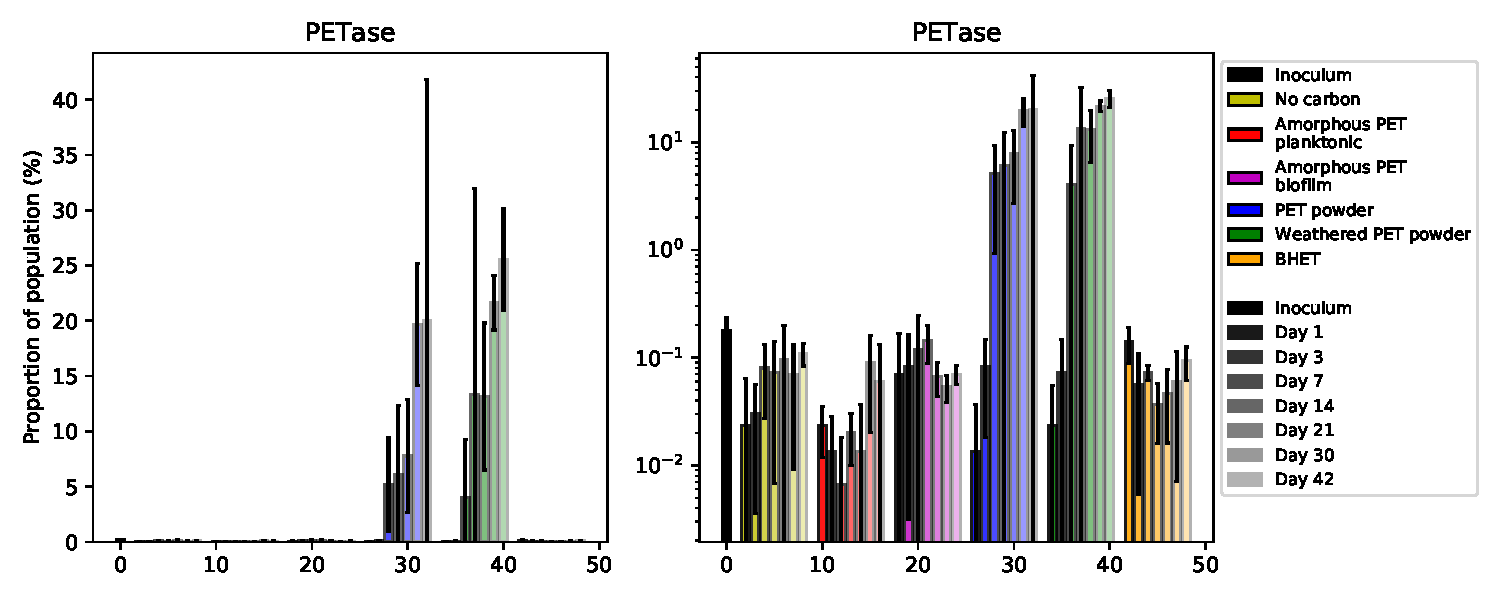
\includegraphics{20-6-15-PET-plastisphere-PICRUSt2_files/figure-latex/plot_raw_PETase-1.pdf}

\hypertarget{tpha2}{%
\subsubsection{tphA2}\label{tpha2}}

\begin{Shaded}
\begin{Highlighting}[]
\NormalTok{plot_picrust_raw(}\StringTok{'tphA2'}\NormalTok{)}
\NormalTok{plt.show()}
\end{Highlighting}
\end{Shaded}

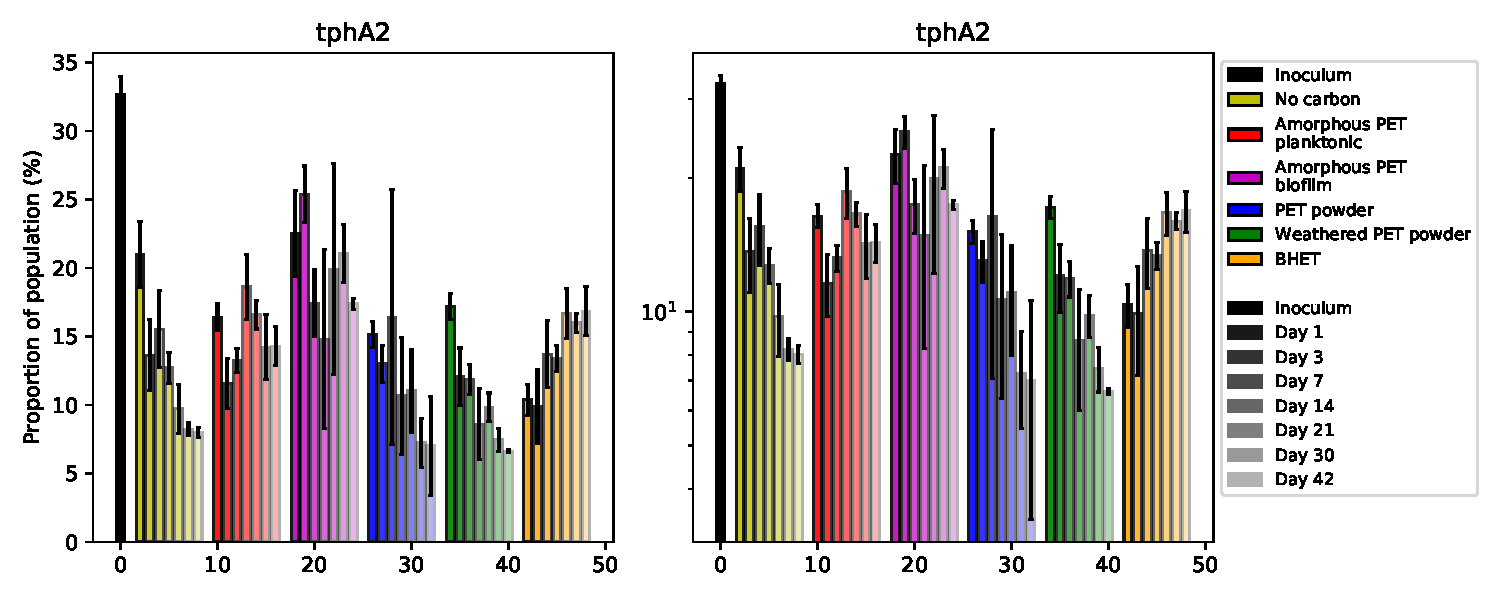
\includegraphics{20-6-15-PET-plastisphere-PICRUSt2_files/figure-latex/plot_raw_tphA2-1.pdf}

\hypertarget{tpha3}{%
\subsubsection{tphA3}\label{tpha3}}

\begin{Shaded}
\begin{Highlighting}[]
\NormalTok{plot_picrust_raw(}\StringTok{'tphA3'}\NormalTok{)}
\NormalTok{plt.show()}
\end{Highlighting}
\end{Shaded}

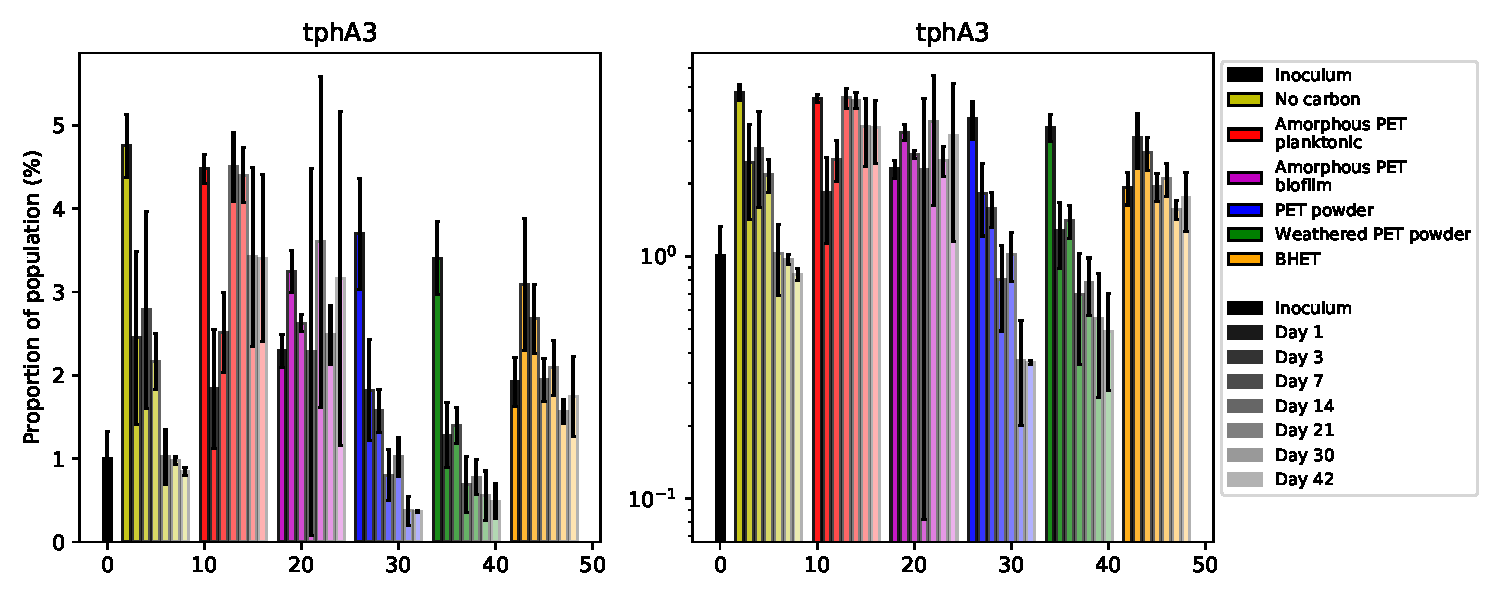
\includegraphics{20-6-15-PET-plastisphere-PICRUSt2_files/figure-latex/plot_raw_tphA3-1.pdf}

\hypertarget{tphb}{%
\subsubsection{tphB}\label{tphb}}

\begin{Shaded}
\begin{Highlighting}[]
\NormalTok{plot_picrust_raw(}\StringTok{'tphB'}\NormalTok{)}
\NormalTok{plt.show()}
\end{Highlighting}
\end{Shaded}

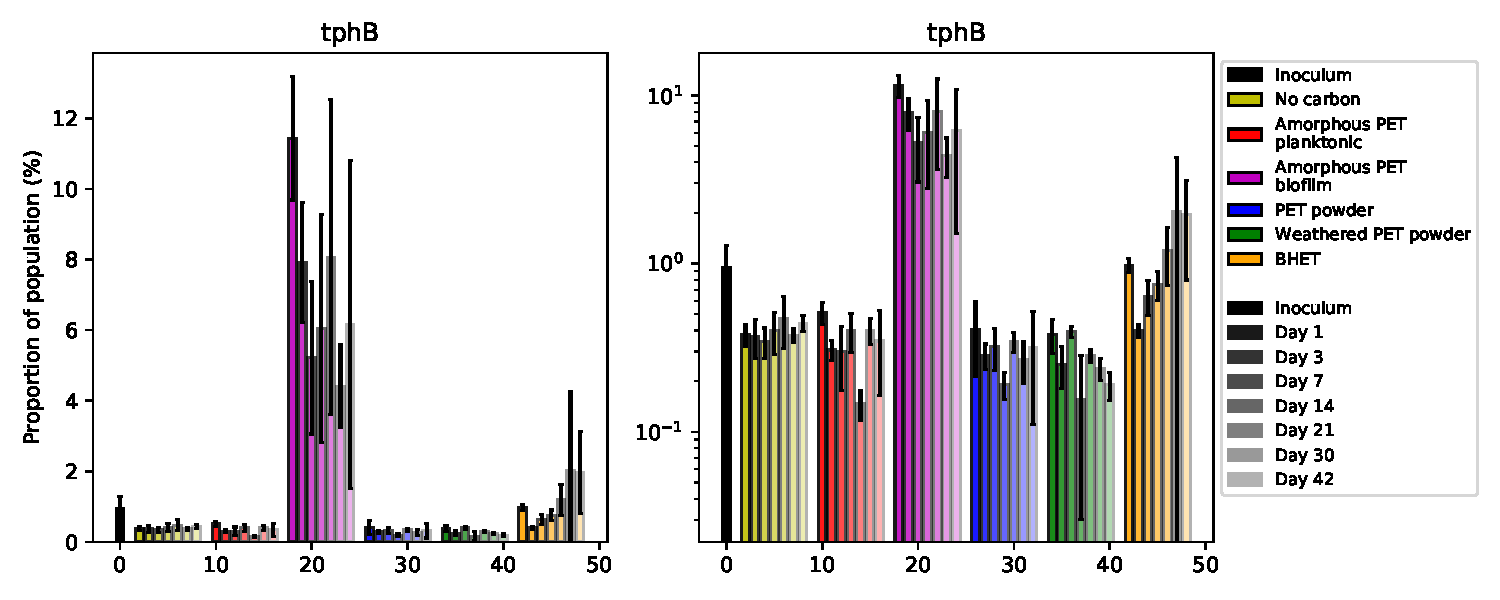
\includegraphics{20-6-15-PET-plastisphere-PICRUSt2_files/figure-latex/plot_raw_tphB-1.pdf}

\hypertarget{k00448}{%
\subsubsection{K00448}\label{k00448}}

\begin{Shaded}
\begin{Highlighting}[]
\NormalTok{plot_picrust_raw(}\StringTok{'K00448'}\NormalTok{)}
\NormalTok{plt.show()}
\end{Highlighting}
\end{Shaded}

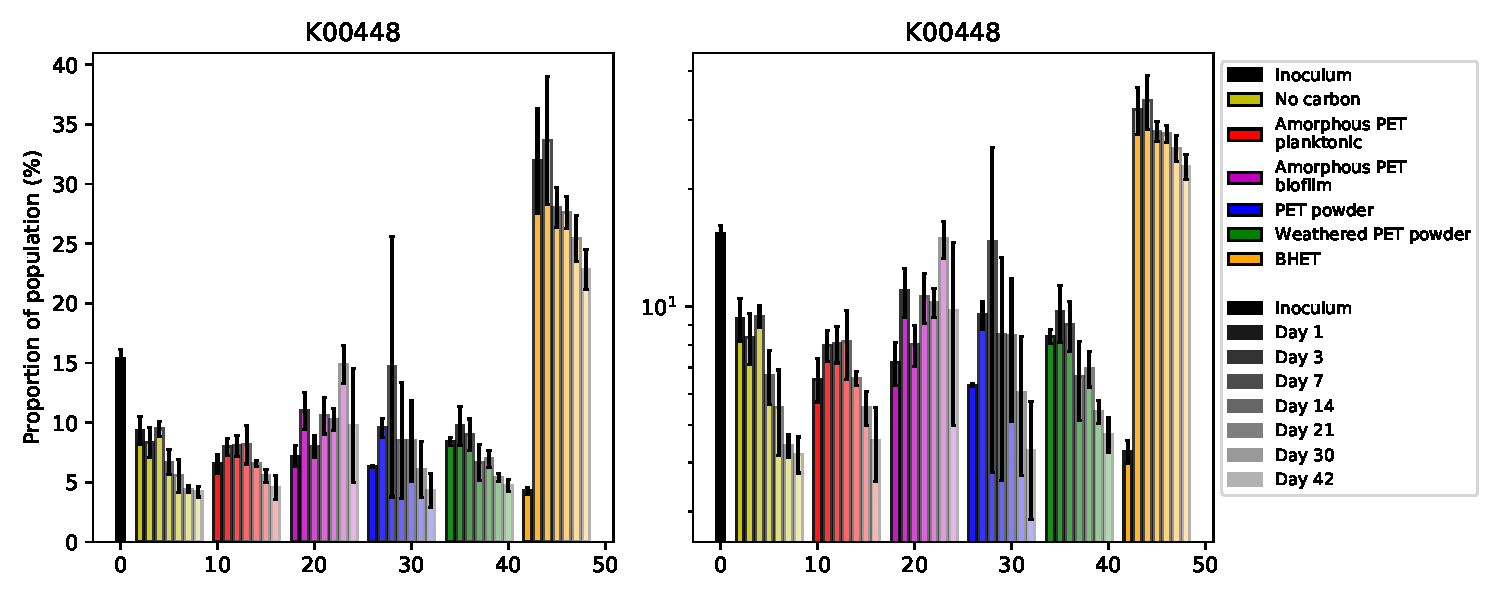
\includegraphics{20-6-15-PET-plastisphere-PICRUSt2_files/figure-latex/plot_raw_K00448-1.pdf}

\hypertarget{k00449}{%
\subsubsection{K00449}\label{k00449}}

\begin{Shaded}
\begin{Highlighting}[]
\NormalTok{plot_picrust_raw(}\StringTok{'K00449'}\NormalTok{)}
\NormalTok{plt.show()}
\end{Highlighting}
\end{Shaded}

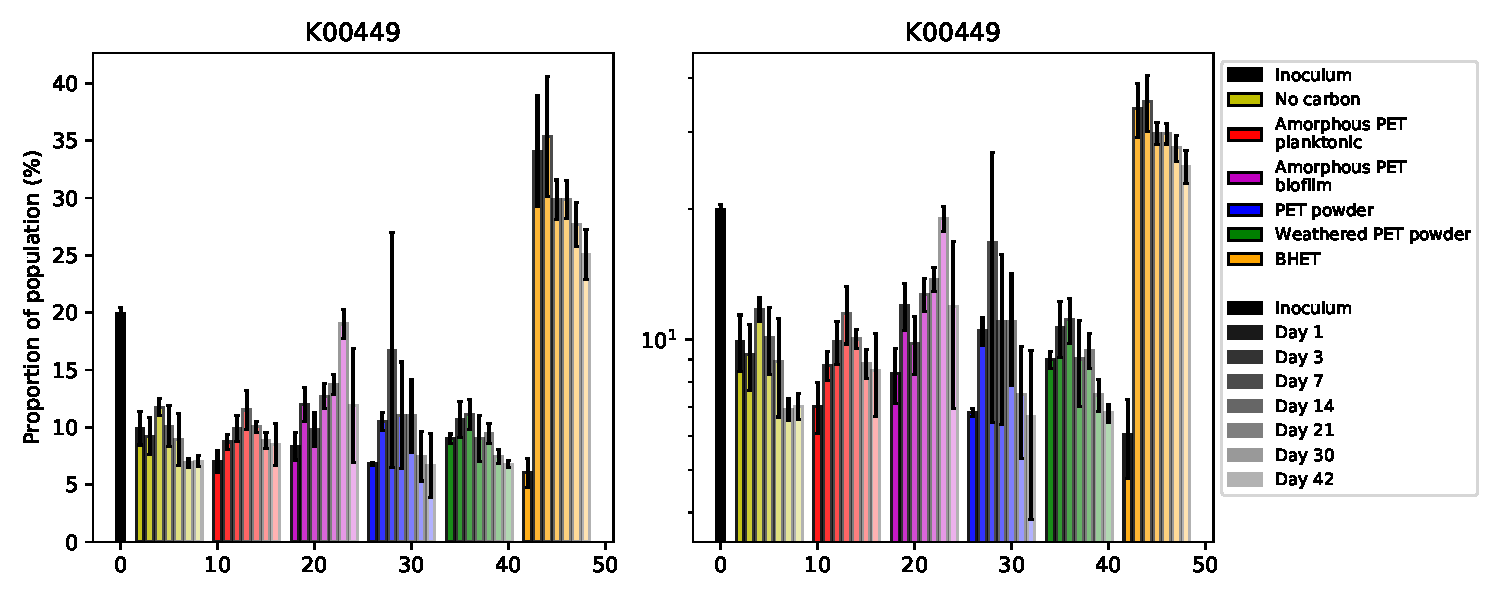
\includegraphics{20-6-15-PET-plastisphere-PICRUSt2_files/figure-latex/plot_raw_K00449-1.pdf}

\hypertarget{k01857}{%
\subsubsection{K01857}\label{k01857}}

\begin{Shaded}
\begin{Highlighting}[]
\NormalTok{plot_picrust_raw(}\StringTok{'K01857'}\NormalTok{)}
\NormalTok{plt.show()}
\end{Highlighting}
\end{Shaded}

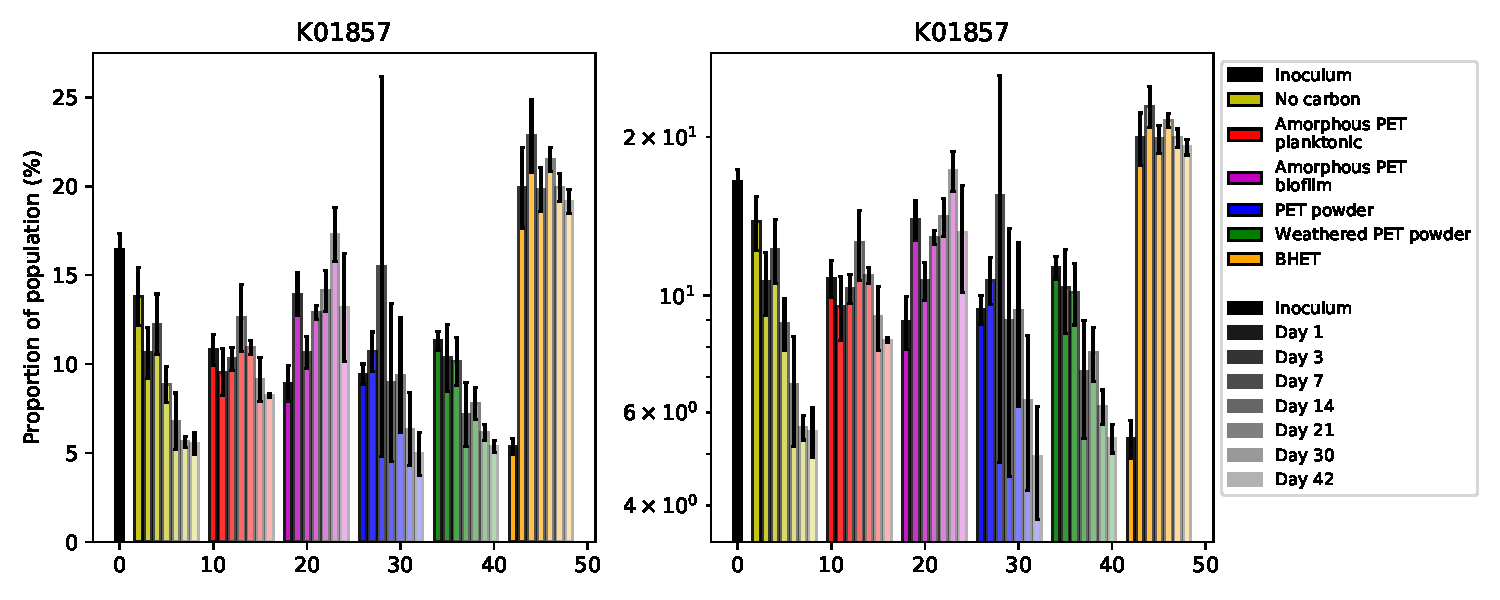
\includegraphics{20-6-15-PET-plastisphere-PICRUSt2_files/figure-latex/plot_raw_K01857-1.pdf}

\hypertarget{k01607}{%
\subsubsection{K01607}\label{k01607}}

\begin{Shaded}
\begin{Highlighting}[]
\NormalTok{plot_picrust_raw(}\StringTok{'K01607'}\NormalTok{)}
\NormalTok{plt.show()}
\end{Highlighting}
\end{Shaded}

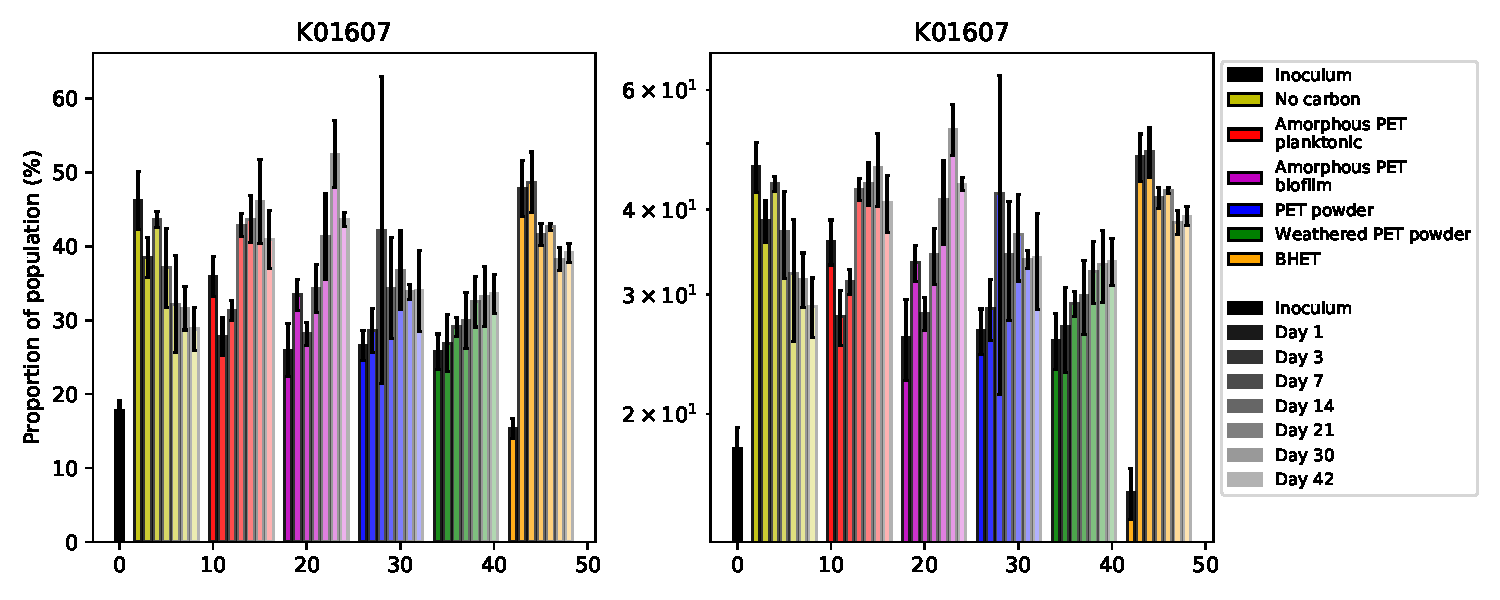
\includegraphics{20-6-15-PET-plastisphere-PICRUSt2_files/figure-latex/plot_raw_K01607-1.pdf}

\hypertarget{k14727}{%
\subsubsection{K14727}\label{k14727}}

\begin{Shaded}
\begin{Highlighting}[]
\NormalTok{plot_picrust_raw(}\StringTok{'K14727'}\NormalTok{)}
\NormalTok{plt.show()}
\end{Highlighting}
\end{Shaded}

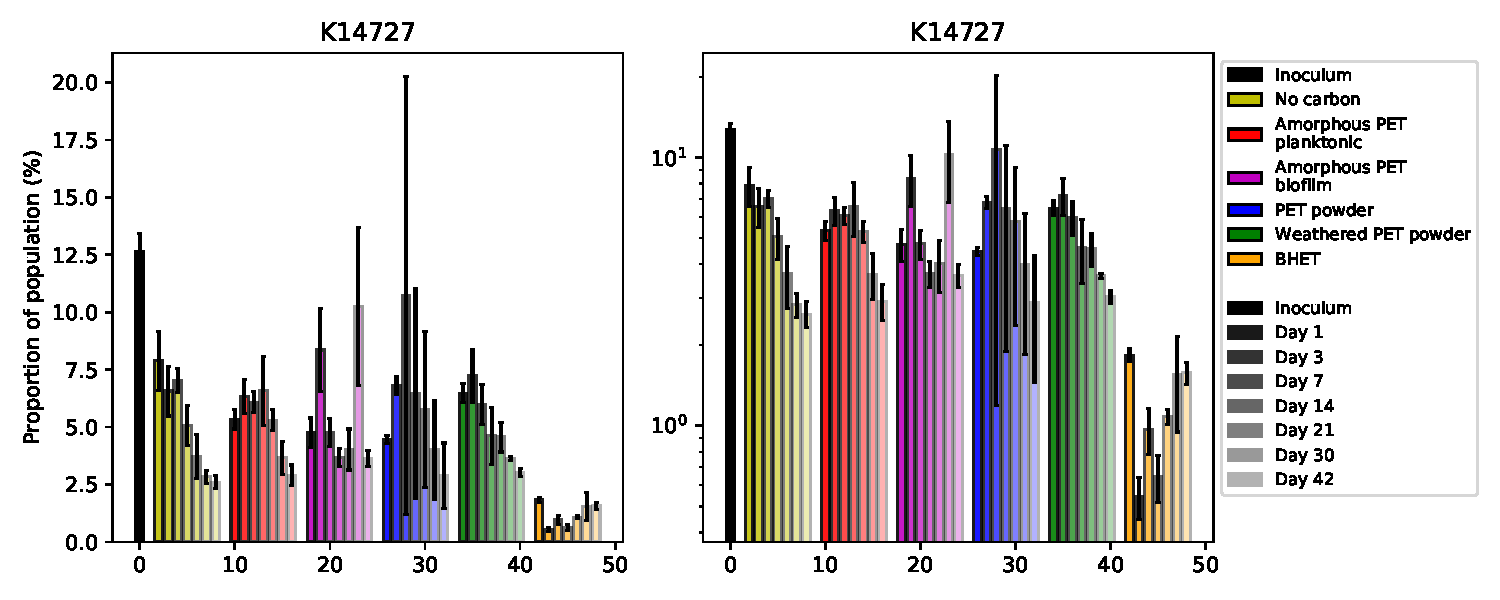
\includegraphics{20-6-15-PET-plastisphere-PICRUSt2_files/figure-latex/plot_raw_K14727-1.pdf}

\hypertarget{k01055}{%
\subsubsection{K01055}\label{k01055}}

\begin{Shaded}
\begin{Highlighting}[]
\NormalTok{plot_picrust_raw(}\StringTok{'K01055'}\NormalTok{)}
\NormalTok{plt.show()}
\end{Highlighting}
\end{Shaded}

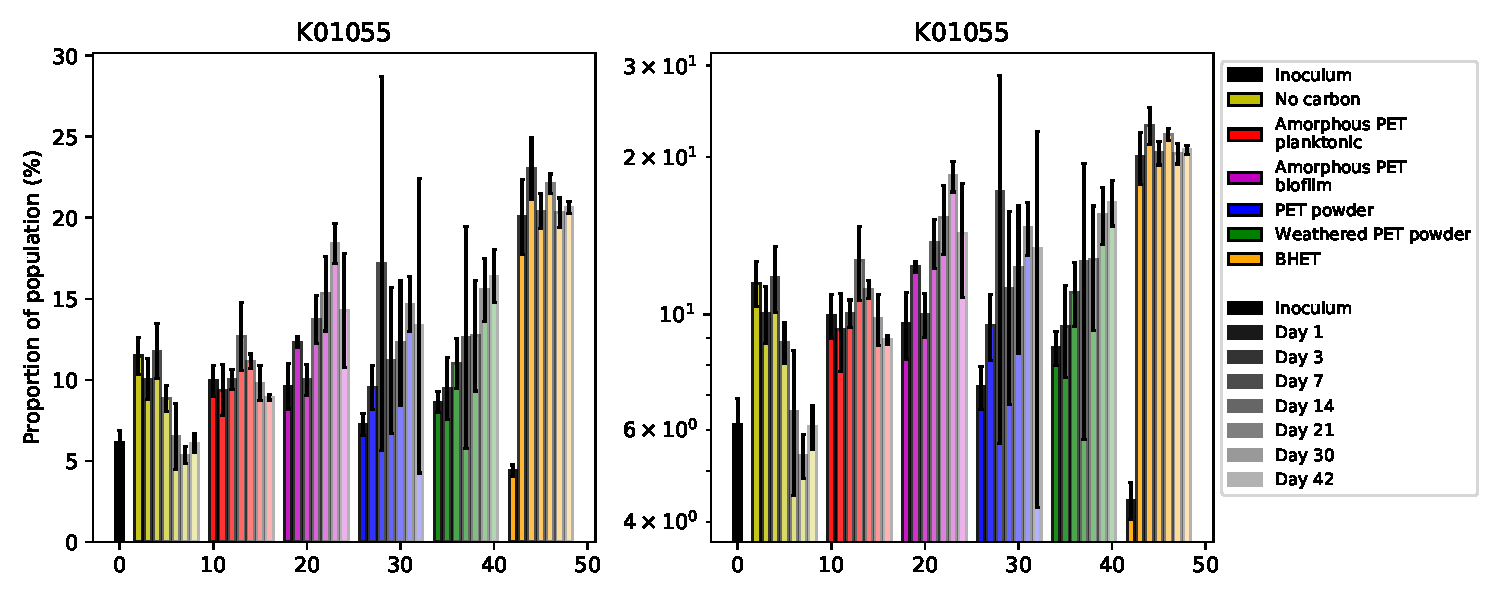
\includegraphics{20-6-15-PET-plastisphere-PICRUSt2_files/figure-latex/plot_raw_K01055-1.pdf}

\hypertarget{k01031}{%
\subsubsection{K01031}\label{k01031}}

\begin{Shaded}
\begin{Highlighting}[]
\NormalTok{plot_picrust_raw(}\StringTok{'K01031'}\NormalTok{)}
\NormalTok{plt.show()}
\end{Highlighting}
\end{Shaded}

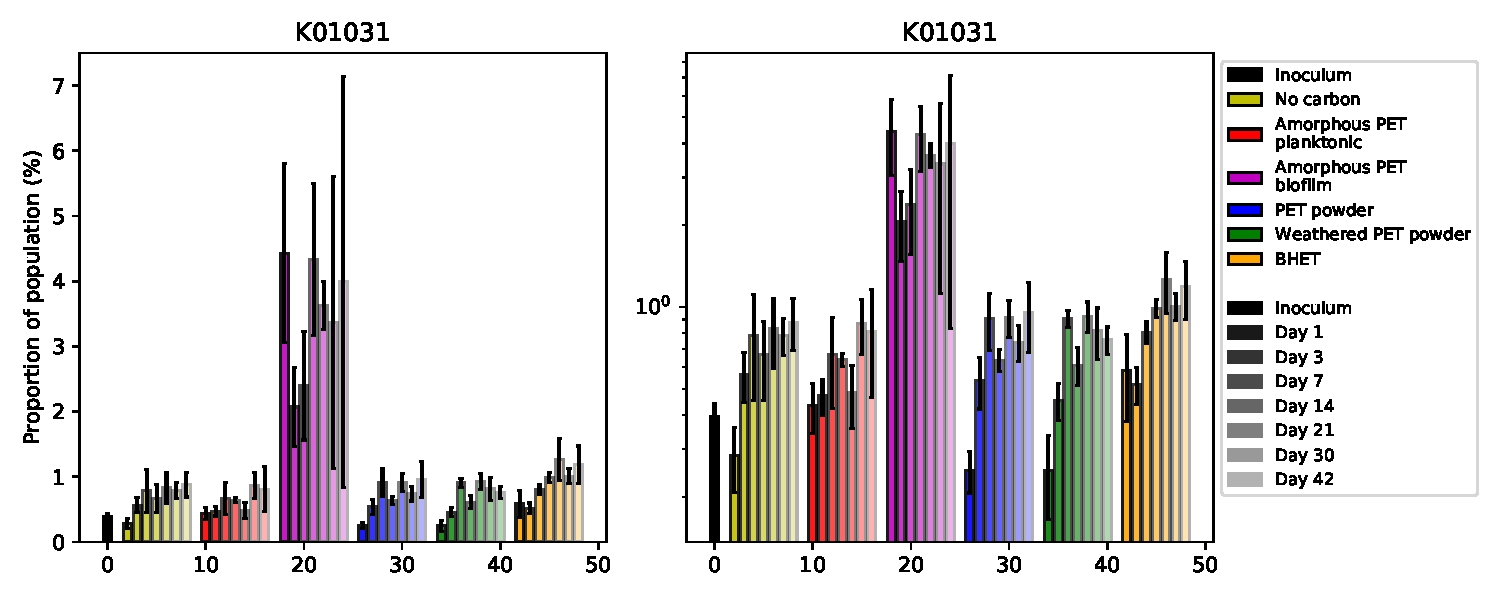
\includegraphics{20-6-15-PET-plastisphere-PICRUSt2_files/figure-latex/plot_raw_K01031-1.pdf}

\hypertarget{k01032}{%
\subsubsection{K01032}\label{k01032}}

\begin{Shaded}
\begin{Highlighting}[]
\NormalTok{plot_picrust_raw(}\StringTok{'K01032'}\NormalTok{)}
\NormalTok{plt.show()}
\end{Highlighting}
\end{Shaded}

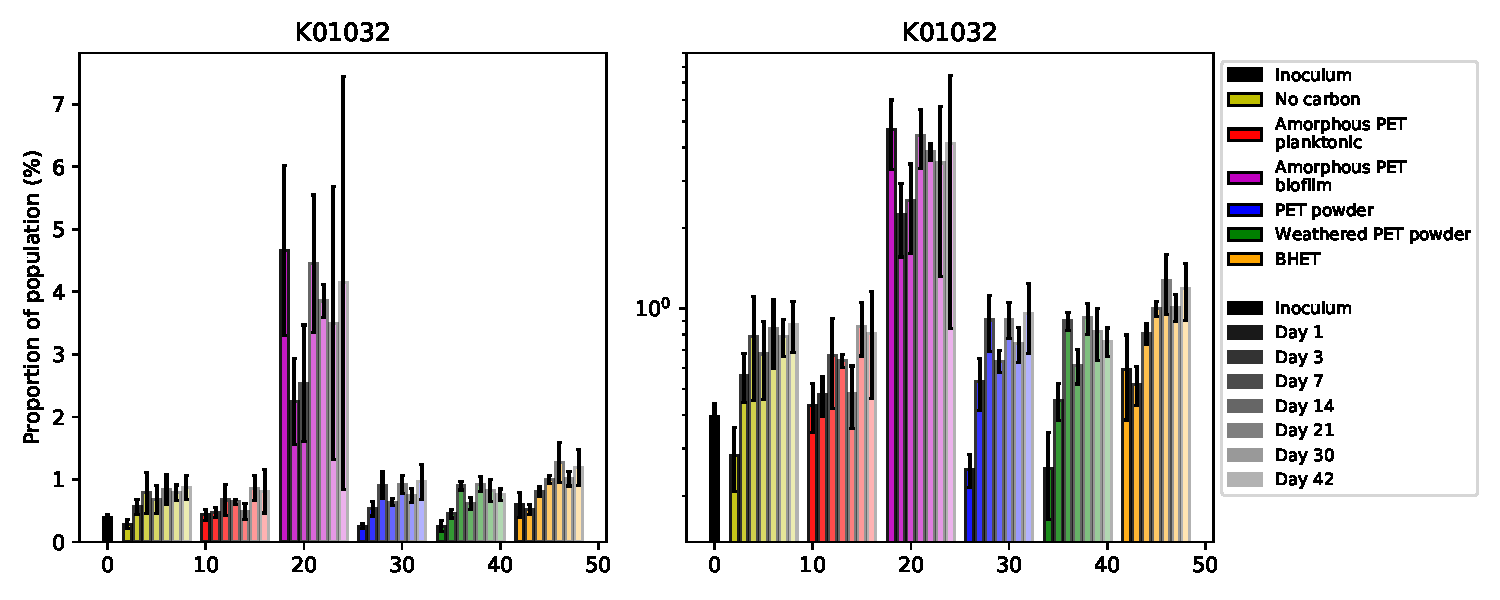
\includegraphics{20-6-15-PET-plastisphere-PICRUSt2_files/figure-latex/plot_raw_K01032-1.pdf}

\hypertarget{fold-change-with-no-carbon-control}{%
\subsection{Fold change with no carbon
control}\label{fold-change-with-no-carbon-control}}

Now I am plotting the Log2 fold change for each K0 compared with the
mean value for the no carbon control.

\begin{Shaded}
\begin{Highlighting}[]
\NormalTok{picrust_unstrat_log }\OperatorTok{=}\NormalTok{ picrust_unstrat.replace(to_replace}\OperatorTok{=}\DecValTok{0}\NormalTok{, value}\OperatorTok{=}\FloatTok{0.00001}\NormalTok{)}
\CommentTok{#math.log2(num)}
\NormalTok{rename }\OperatorTok{=}\NormalTok{ \{\}}
\ControlFlowTok{for}\NormalTok{ col }\KeywordTok{in} \BuiltInTok{list}\NormalTok{(picrust_unstrat.columns):}
  \ControlFlowTok{if} \StringTok{'NoC'} \KeywordTok{in}\NormalTok{ col:}
\NormalTok{    rename[col] }\OperatorTok{=} \StringTok{'NoC'}
\NormalTok{picrust_unstrat_log.rename(columns}\OperatorTok{=}\NormalTok{rename, inplace}\OperatorTok{=}\VariableTok{True}\NormalTok{)}
\KeywordTok{def}\NormalTok{ get_fc(function):}
\NormalTok{  ma, mi }\OperatorTok{=} \DecValTok{0}\NormalTok{, }\DecValTok{0}
\NormalTok{  this_abun }\OperatorTok{=}\NormalTok{ pd.DataFrame(picrust_unstrat_log.loc[function, :])}
\NormalTok{  x, y }\OperatorTok{=}\NormalTok{ [}\DecValTok{0}\NormalTok{, }\DecValTok{1}\NormalTok{, }\DecValTok{2}\NormalTok{, }\DecValTok{3}\NormalTok{, }\DecValTok{4}\NormalTok{, }\DecValTok{5}\NormalTok{, }\DecValTok{6}\NormalTok{, }\DecValTok{7}\NormalTok{, }\DecValTok{1}\NormalTok{, }\DecValTok{2}\NormalTok{, }\DecValTok{3}\NormalTok{, }\DecValTok{4}\NormalTok{, }\DecValTok{5}\NormalTok{, }\DecValTok{6}\NormalTok{, }\DecValTok{7}\NormalTok{, }\DecValTok{1}\NormalTok{, }\DecValTok{2}\NormalTok{, }\DecValTok{3}\NormalTok{, }\DecValTok{4}\NormalTok{, }\DecValTok{5}\NormalTok{, }\DecValTok{6}\NormalTok{, }\DecValTok{7}\NormalTok{, }\DecValTok{1}\NormalTok{, }\DecValTok{2}\NormalTok{, }\DecValTok{3}\NormalTok{, }\DecValTok{4}\NormalTok{, }\DecValTok{5}\NormalTok{, }\DecValTok{6}\NormalTok{, }\DecValTok{7}\NormalTok{, }\DecValTok{1}\NormalTok{, }\DecValTok{2}\NormalTok{, }\DecValTok{3}\NormalTok{, }\DecValTok{4}\NormalTok{, }\DecValTok{5}\NormalTok{, }\DecValTok{6}\NormalTok{, }\DecValTok{7}\NormalTok{, ], [}\DecValTok{0}\NormalTok{, }\DecValTok{4}\NormalTok{, }\DecValTok{4}\NormalTok{, }\DecValTok{4}\NormalTok{, }\DecValTok{4}\NormalTok{, }\DecValTok{4}\NormalTok{, }\DecValTok{4}\NormalTok{, }\DecValTok{4}\NormalTok{, }\DecValTok{3}\NormalTok{, }\DecValTok{3}\NormalTok{, }\DecValTok{3}\NormalTok{, }\DecValTok{3}\NormalTok{, }\DecValTok{3}\NormalTok{, }\DecValTok{3}\NormalTok{, }\DecValTok{3}\NormalTok{, }\DecValTok{2}\NormalTok{, }\DecValTok{2}\NormalTok{, }\DecValTok{2}\NormalTok{, }\DecValTok{2}\NormalTok{, }\DecValTok{2}\NormalTok{, }\DecValTok{2}\NormalTok{, }\DecValTok{2}\NormalTok{, }\DecValTok{1}\NormalTok{, }\DecValTok{1}\NormalTok{, }\DecValTok{1}\NormalTok{, }\DecValTok{1}\NormalTok{, }\DecValTok{1}\NormalTok{, }\DecValTok{1}\NormalTok{, }\DecValTok{1}\NormalTok{, }\DecValTok{0}\NormalTok{, }\DecValTok{0}\NormalTok{, }\DecValTok{0}\NormalTok{, }\DecValTok{0}\NormalTok{, }\DecValTok{0}\NormalTok{, }\DecValTok{0}\NormalTok{, }\DecValTok{0}\NormalTok{]}
\NormalTok{  plt.figure(figsize}\OperatorTok{=}\NormalTok{(}\DecValTok{3}\NormalTok{,}\DecValTok{3}\NormalTok{))}
\NormalTok{  ax1 }\OperatorTok{=}\NormalTok{ plt.subplot(}\DecValTok{111}\NormalTok{)}
\NormalTok{  nc }\OperatorTok{=}\NormalTok{ this_abun.loc[}\StringTok{'NoC'}\NormalTok{, :].mean()}
  \BuiltInTok{print}\NormalTok{(nc)}
\NormalTok{  nc }\OperatorTok{=}\NormalTok{ math.log2(nc)}
\NormalTok{  new_order }\OperatorTok{=}\NormalTok{ []}
  \ControlFlowTok{for}\NormalTok{ sample }\KeywordTok{in}\NormalTok{ sample_order:}
    \ControlFlowTok{if} \StringTok{'NoC'} \KeywordTok{not} \KeywordTok{in}\NormalTok{ sample:}
\NormalTok{      new_order.append(sample)}
\NormalTok{  colormap, norm }\OperatorTok{=}\NormalTok{ mpl.cm.get_cmap(}\StringTok{'RdBu_r'}\NormalTok{, }\DecValTok{256}\NormalTok{), mpl.colors.Normalize(vmin}\OperatorTok{=-}\DecValTok{10}\NormalTok{, vmax}\OperatorTok{=}\DecValTok{10}\NormalTok{)}
\NormalTok{  m }\OperatorTok{=}\NormalTok{ mpl.cm.ScalarMappable(norm}\OperatorTok{=}\NormalTok{norm, cmap}\OperatorTok{=}\NormalTok{colormap)}
\NormalTok{  ax1 }\OperatorTok{=}\NormalTok{ plt.subplot2grid((}\DecValTok{7}\NormalTok{,}\DecValTok{8}\NormalTok{), (}\DecValTok{2}\NormalTok{,}\DecValTok{1}\NormalTok{), rowspan}\OperatorTok{=}\DecValTok{5}\NormalTok{, colspan}\OperatorTok{=}\DecValTok{7}\NormalTok{)}
\NormalTok{  axinoc }\OperatorTok{=}\NormalTok{ plt.subplot2grid((}\DecValTok{7}\NormalTok{,}\DecValTok{8}\NormalTok{), (}\DecValTok{4}\NormalTok{,}\DecValTok{0}\NormalTok{))}
\NormalTok{  axcolbar }\OperatorTok{=}\NormalTok{ plt.subplot2grid((}\DecValTok{7}\NormalTok{,}\DecValTok{8}\NormalTok{), (}\DecValTok{0}\NormalTok{,}\DecValTok{1}\NormalTok{), colspan}\OperatorTok{=}\DecValTok{7}\NormalTok{, frameon}\OperatorTok{=}\VariableTok{False}\NormalTok{)}
\NormalTok{  plt.sca(axcolbar)}
\NormalTok{  plt.xticks([]), plt.yticks([])}
  \ControlFlowTok{for}\NormalTok{ a }\KeywordTok{in} \BuiltInTok{range}\NormalTok{(}\BuiltInTok{len}\NormalTok{(new_order)):}
\NormalTok{    this_mean_abs }\OperatorTok{=}\NormalTok{ this_abun.loc[new_order[a], :].mean()}
\NormalTok{    this_mean }\OperatorTok{=}\NormalTok{ math.log2(this_mean_abs)}
\NormalTok{    this_diff }\OperatorTok{=}\NormalTok{ math.}\BuiltInTok{pow}\NormalTok{(this_mean}\OperatorTok{-}\NormalTok{nc, }\DecValTok{2}\NormalTok{)}
    \ControlFlowTok{if}\NormalTok{ this_diff }\OperatorTok{<} \DecValTok{1}\NormalTok{:}
\NormalTok{      this_diff }\OperatorTok{=} \DecValTok{-1}\OperatorTok{/}\NormalTok{this_diff}
    \CommentTok{#print(new_order[a], float(nc), float(this_mean_abs), float(this_diff), '\textbackslash{}n')}
\NormalTok{    color }\OperatorTok{=}\NormalTok{ m.to_rgba(this_diff)}
    \ControlFlowTok{if}\NormalTok{ this_diff }\OperatorTok{>}\NormalTok{ ma: ma }\OperatorTok{=}\NormalTok{ this_diff}
    \ControlFlowTok{if}\NormalTok{ this_diff }\OperatorTok{<}\NormalTok{ mi: mi }\OperatorTok{=}\NormalTok{ this_diff}
    \ControlFlowTok{if}\NormalTok{ x[a] }\OperatorTok{==} \DecValTok{0} \KeywordTok{and}\NormalTok{ y[a] }\OperatorTok{==} \DecValTok{0}\NormalTok{:}
\NormalTok{      axinoc.bar([}\DecValTok{1}\NormalTok{], [}\DecValTok{1}\NormalTok{], color}\OperatorTok{=}\NormalTok{color, edgecolor}\OperatorTok{=}\StringTok{'k'}\NormalTok{, width}\OperatorTok{=}\DecValTok{1}\NormalTok{)}
\NormalTok{      axinoc.set_xlim([}\FloatTok{0.5}\NormalTok{, }\FloatTok{1.5}\NormalTok{]), axinoc.set_ylim([}\DecValTok{0}\NormalTok{,}\DecValTok{1}\NormalTok{])}
      \BuiltInTok{print}\NormalTok{(new_order[a])}
    \ControlFlowTok{else}\NormalTok{:}
\NormalTok{      ax1.bar([x[a]], [}\DecValTok{1}\NormalTok{], bottom}\OperatorTok{=}\NormalTok{[y[a]], color}\OperatorTok{=}\NormalTok{color, edgecolor}\OperatorTok{=}\StringTok{'k'}\NormalTok{, width}\OperatorTok{=}\DecValTok{1}\NormalTok{)}
  \BuiltInTok{print}\NormalTok{(new_order)}
\NormalTok{  plt.sca(ax1)}
\NormalTok{  plt.xticks([}\DecValTok{1}\NormalTok{, }\DecValTok{2}\NormalTok{, }\DecValTok{3}\NormalTok{, }\DecValTok{4}\NormalTok{, }\DecValTok{5}\NormalTok{, }\DecValTok{6}\NormalTok{, }\DecValTok{7}\NormalTok{], [}\StringTok{'Day 1'}\NormalTok{, }\StringTok{'Day 3'}\NormalTok{, }\StringTok{'Day 7'}\NormalTok{, }\StringTok{'Day 14'}\NormalTok{, }\StringTok{'Day 21'}\NormalTok{, }\StringTok{'Day 30'}\NormalTok{, }\StringTok{'Day 42'}\NormalTok{], rotation}\OperatorTok{=}\DecValTok{90}\NormalTok{)}
\NormalTok{  plt.yticks([}\FloatTok{0.5}\NormalTok{, }\FloatTok{1.5}\NormalTok{, }\FloatTok{2.5}\NormalTok{, }\FloatTok{3.5}\NormalTok{, }\FloatTok{4.5}\NormalTok{, }\FloatTok{5.5}\NormalTok{], [}\StringTok{'BHET'}\NormalTok{, }\StringTok{'Weathered}\CharTok{\textbackslash{}n}\StringTok{PET powder'}\NormalTok{, }\StringTok{'PET powder'}\NormalTok{, }\StringTok{'Amorphous PET}\CharTok{\textbackslash{}n}\StringTok{Biofilm'}\NormalTok{, }\StringTok{'Amorphous PET}\CharTok{\textbackslash{}n}\StringTok{Planktonic'}\NormalTok{])}
\NormalTok{  ax1.yaxis.set_ticks_position(}\StringTok{'right'}\NormalTok{)}
\NormalTok{  plt.sca(axinoc)}
\NormalTok{  plt.xticks([}\DecValTok{1}\NormalTok{], [}\StringTok{'Inoculum'}\NormalTok{], rotation}\OperatorTok{=}\DecValTok{90}\NormalTok{)}
\NormalTok{  plt.yticks([])}
\NormalTok{  ax1.set_xlim([}\FloatTok{0.5}\NormalTok{, }\FloatTok{7.5}\NormalTok{]), ax1.set_ylim([}\DecValTok{0}\NormalTok{, }\DecValTok{5}\NormalTok{])}
\NormalTok{  cb1 }\OperatorTok{=}\NormalTok{ mpl.colorbar.ColorbarBase(axcolbar, cmap}\OperatorTok{=}\NormalTok{colormap, norm}\OperatorTok{=}\NormalTok{norm, orientation}\OperatorTok{=}\StringTok{'horizontal'}\NormalTok{)}
\NormalTok{  cb1.set_ticks([])}
\NormalTok{  axcolbar.text(}\OperatorTok{-}\DecValTok{12}\NormalTok{, }\DecValTok{-22}\NormalTok{, }\StringTok{'<-10'}\NormalTok{)}
\NormalTok{  axcolbar.text(}\DecValTok{9}\NormalTok{, }\DecValTok{-22}\NormalTok{, }\StringTok{'>10'}\NormalTok{)}
\NormalTok{  axcolbar.text(}\DecValTok{0}\NormalTok{, }\DecValTok{0}\NormalTok{, }\StringTok{'Fold change'}\NormalTok{, ha}\OperatorTok{=}\StringTok{'center'}\NormalTok{, va}\OperatorTok{=}\StringTok{'center'}\NormalTok{)}
\NormalTok{  plt.tight_layout()}
\end{Highlighting}
\end{Shaded}

\hypertarget{petase-1}{%
\subsubsection{PETase}\label{petase-1}}

\begin{Shaded}
\begin{Highlighting}[]
\NormalTok{get_fc(}\StringTok{'PETase'}\NormalTok{)}
\end{Highlighting}
\end{Shaded}

\begin{Shaded}
\begin{Highlighting}[]
\NormalTok{plt.tight_layout()}
\end{Highlighting}
\end{Shaded}

\begin{Shaded}
\begin{Highlighting}[]
\NormalTok{plt.show()}
\end{Highlighting}
\end{Shaded}

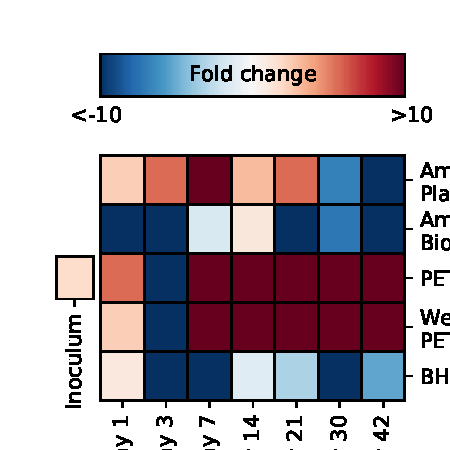
\includegraphics{20-6-15-PET-plastisphere-PICRUSt2_files/figure-latex/plot_fc_petase-1.pdf}

\hypertarget{tpha2-1}{%
\subsubsection{tphA2}\label{tpha2-1}}

\begin{Shaded}
\begin{Highlighting}[]
\NormalTok{get_fc(}\StringTok{'tphA2'}\NormalTok{)}
\end{Highlighting}
\end{Shaded}

\begin{Shaded}
\begin{Highlighting}[]
\NormalTok{plt.tight_layout()}
\end{Highlighting}
\end{Shaded}

\begin{Shaded}
\begin{Highlighting}[]
\NormalTok{plt.show()}
\end{Highlighting}
\end{Shaded}

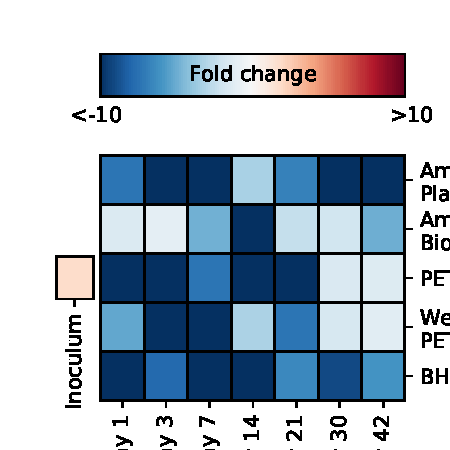
\includegraphics{20-6-15-PET-plastisphere-PICRUSt2_files/figure-latex/plot_fc_tphA2-1.pdf}

\hypertarget{tpha3-1}{%
\subsubsection{tphA3}\label{tpha3-1}}

\begin{Shaded}
\begin{Highlighting}[]
\NormalTok{get_fc(}\StringTok{'tphA3'}\NormalTok{)}
\end{Highlighting}
\end{Shaded}

\begin{Shaded}
\begin{Highlighting}[]
\NormalTok{plt.tight_layout()}
\end{Highlighting}
\end{Shaded}

\begin{Shaded}
\begin{Highlighting}[]
\NormalTok{plt.show()}
\end{Highlighting}
\end{Shaded}

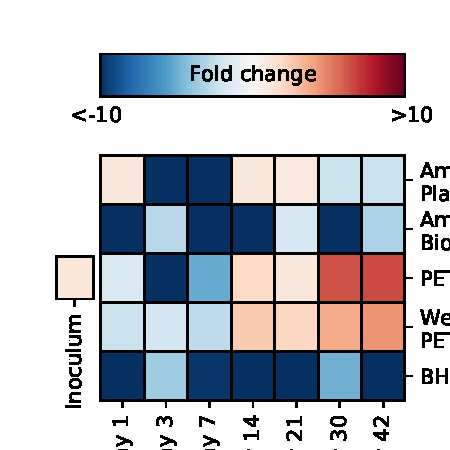
\includegraphics{20-6-15-PET-plastisphere-PICRUSt2_files/figure-latex/plot_fc_tphA3-1.pdf}

\hypertarget{tphb-1}{%
\subsubsection{tphB}\label{tphb-1}}

\begin{Shaded}
\begin{Highlighting}[]
\NormalTok{get_fc(}\StringTok{'tphB'}\NormalTok{)}
\end{Highlighting}
\end{Shaded}

\begin{Shaded}
\begin{Highlighting}[]
\NormalTok{plt.tight_layout()}
\end{Highlighting}
\end{Shaded}

\begin{Shaded}
\begin{Highlighting}[]
\NormalTok{plt.show()}
\end{Highlighting}
\end{Shaded}

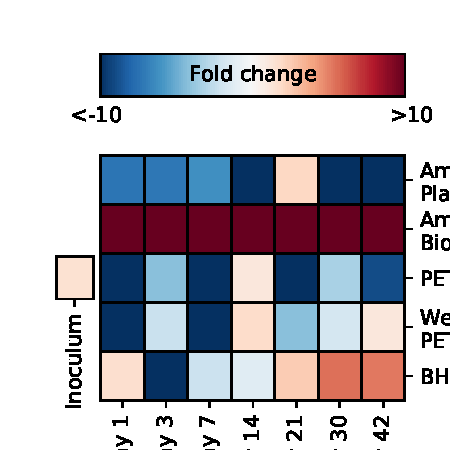
\includegraphics{20-6-15-PET-plastisphere-PICRUSt2_files/figure-latex/plot_fc_tphB-1.pdf}

\hypertarget{k00448-1}{%
\subsubsection{K00448}\label{k00448-1}}

\begin{Shaded}
\begin{Highlighting}[]
\NormalTok{get_fc(}\StringTok{'K00448'}\NormalTok{)}
\end{Highlighting}
\end{Shaded}

\begin{Shaded}
\begin{Highlighting}[]
\NormalTok{plt.tight_layout()}
\end{Highlighting}
\end{Shaded}

\begin{Shaded}
\begin{Highlighting}[]
\NormalTok{plt.show()}
\end{Highlighting}
\end{Shaded}

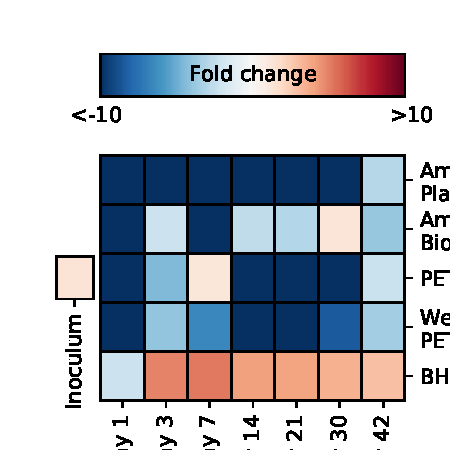
\includegraphics{20-6-15-PET-plastisphere-PICRUSt2_files/figure-latex/plot_fc_K00448-1.pdf}

\hypertarget{k00449-1}{%
\subsubsection{K00449}\label{k00449-1}}

\begin{Shaded}
\begin{Highlighting}[]
\NormalTok{get_fc(}\StringTok{'K00449'}\NormalTok{)}
\end{Highlighting}
\end{Shaded}

\begin{Shaded}
\begin{Highlighting}[]
\NormalTok{plt.tight_layout()}
\end{Highlighting}
\end{Shaded}

\begin{Shaded}
\begin{Highlighting}[]
\NormalTok{plt.show()}
\end{Highlighting}
\end{Shaded}

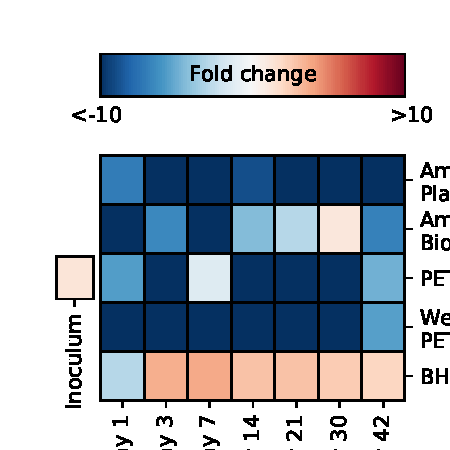
\includegraphics{20-6-15-PET-plastisphere-PICRUSt2_files/figure-latex/plot_fc_K00449-1.pdf}

\hypertarget{k01857-1}{%
\subsubsection{K01857}\label{k01857-1}}

\begin{Shaded}
\begin{Highlighting}[]
\NormalTok{get_fc(}\StringTok{'K01857'}\NormalTok{)}
\end{Highlighting}
\end{Shaded}

\begin{Shaded}
\begin{Highlighting}[]
\NormalTok{plt.tight_layout()}
\end{Highlighting}
\end{Shaded}

\begin{Shaded}
\begin{Highlighting}[]
\NormalTok{plt.show()}
\end{Highlighting}
\end{Shaded}

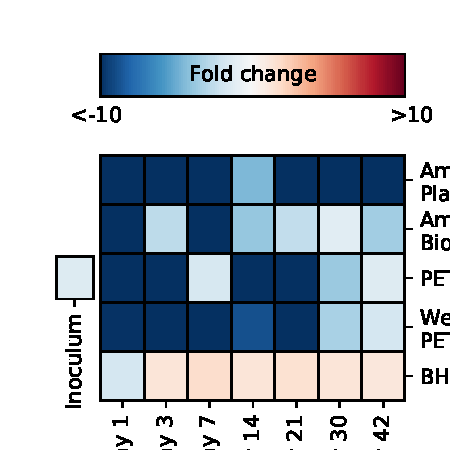
\includegraphics{20-6-15-PET-plastisphere-PICRUSt2_files/figure-latex/plot_fc_K01857-1.pdf}

\hypertarget{k01607-1}{%
\subsubsection{K01607}\label{k01607-1}}

\begin{Shaded}
\begin{Highlighting}[]
\NormalTok{get_fc(}\StringTok{'K01607'}\NormalTok{)}
\end{Highlighting}
\end{Shaded}

\begin{Shaded}
\begin{Highlighting}[]
\NormalTok{plt.tight_layout()}
\end{Highlighting}
\end{Shaded}

\begin{Shaded}
\begin{Highlighting}[]
\NormalTok{plt.show()}
\end{Highlighting}
\end{Shaded}

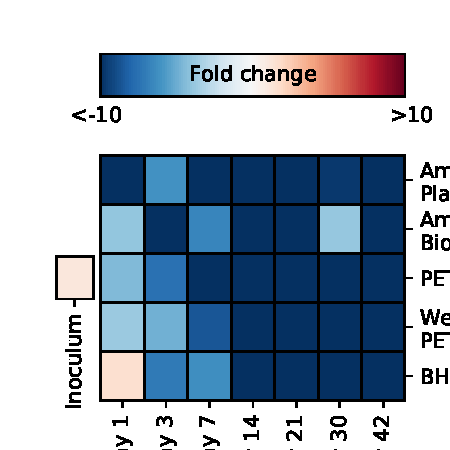
\includegraphics{20-6-15-PET-plastisphere-PICRUSt2_files/figure-latex/plot_fc_K01607-1.pdf}

\hypertarget{k14727-1}{%
\subsubsection{K14727}\label{k14727-1}}

\begin{Shaded}
\begin{Highlighting}[]
\NormalTok{get_fc(}\StringTok{'K14727'}\NormalTok{)}
\end{Highlighting}
\end{Shaded}

\begin{Shaded}
\begin{Highlighting}[]
\NormalTok{plt.tight_layout()}
\end{Highlighting}
\end{Shaded}

\begin{Shaded}
\begin{Highlighting}[]
\NormalTok{plt.show()}
\end{Highlighting}
\end{Shaded}

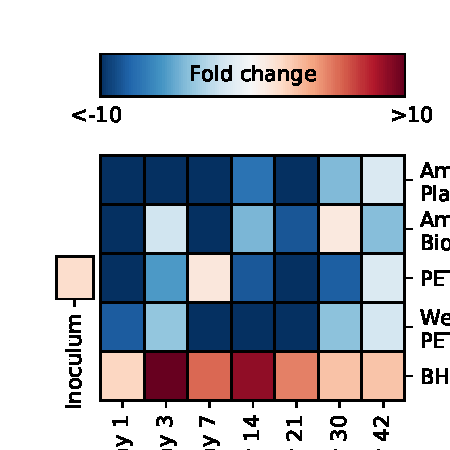
\includegraphics{20-6-15-PET-plastisphere-PICRUSt2_files/figure-latex/plot_fc_K14727-1.pdf}

\hypertarget{k01055-1}{%
\subsubsection{K01055}\label{k01055-1}}

\begin{Shaded}
\begin{Highlighting}[]
\NormalTok{get_fc(}\StringTok{'K01055'}\NormalTok{)}
\end{Highlighting}
\end{Shaded}

\begin{Shaded}
\begin{Highlighting}[]
\NormalTok{plt.tight_layout()}
\end{Highlighting}
\end{Shaded}

\begin{Shaded}
\begin{Highlighting}[]
\NormalTok{plt.show()}
\end{Highlighting}
\end{Shaded}

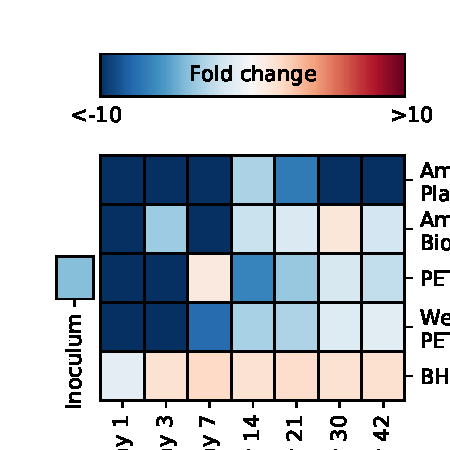
\includegraphics{20-6-15-PET-plastisphere-PICRUSt2_files/figure-latex/plot_fc_K01055-1.pdf}

\hypertarget{k01031-1}{%
\subsubsection{K01031}\label{k01031-1}}

\begin{Shaded}
\begin{Highlighting}[]
\NormalTok{get_fc(}\StringTok{'K01031'}\NormalTok{)}
\end{Highlighting}
\end{Shaded}

\begin{Shaded}
\begin{Highlighting}[]
\NormalTok{plt.tight_layout()}
\end{Highlighting}
\end{Shaded}

\begin{Shaded}
\begin{Highlighting}[]
\NormalTok{plt.show()}
\end{Highlighting}
\end{Shaded}

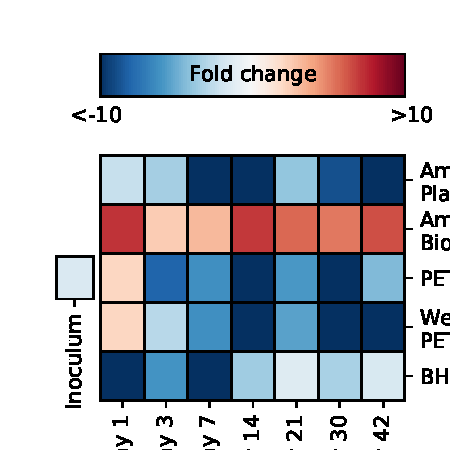
\includegraphics{20-6-15-PET-plastisphere-PICRUSt2_files/figure-latex/plot_fc_K01031-1.pdf}

\hypertarget{k01032-1}{%
\subsubsection{K01032}\label{k01032-1}}

\begin{Shaded}
\begin{Highlighting}[]
\NormalTok{get_fc(}\StringTok{'K01032'}\NormalTok{)}
\end{Highlighting}
\end{Shaded}

\begin{Shaded}
\begin{Highlighting}[]
\NormalTok{plt.tight_layout()}
\end{Highlighting}
\end{Shaded}

\begin{Shaded}
\begin{Highlighting}[]
\NormalTok{plt.show()}
\end{Highlighting}
\end{Shaded}

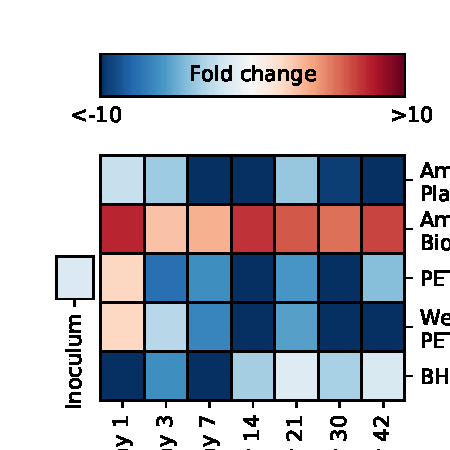
\includegraphics{20-6-15-PET-plastisphere-PICRUSt2_files/figure-latex/plot_fc_K01032-1.pdf}

\hypertarget{key-functions-contribution-by-different-taxa}{%
\subsection{Key functions contribution by different
taxa}\label{key-functions-contribution-by-different-taxa}}

\end{document}
